\documentclass[twoside]{book}

% Packages required by doxygen
\usepackage{fixltx2e}
\usepackage{calc}
\usepackage{doxygen}
\usepackage[export]{adjustbox} % also loads graphicx
\usepackage{graphicx}
\usepackage[utf8]{inputenc}
\usepackage{makeidx}
\usepackage{multicol}
\usepackage{multirow}
\PassOptionsToPackage{warn}{textcomp}
\usepackage{textcomp}
\usepackage[nointegrals]{wasysym}
\usepackage[table]{xcolor}

% Font selection
\usepackage[T1]{fontenc}
\usepackage[scaled=.90]{helvet}
\usepackage{courier}
\usepackage{amssymb}
\usepackage{sectsty}
\renewcommand{\familydefault}{\sfdefault}
\allsectionsfont{%
  \fontseries{bc}\selectfont%
  \color{darkgray}%
}
\renewcommand{\DoxyLabelFont}{%
  \fontseries{bc}\selectfont%
  \color{darkgray}%
}
\newcommand{\+}{\discretionary{\mbox{\scriptsize$\hookleftarrow$}}{}{}}

% Page & text layout
\usepackage{geometry}
\geometry{%
  a4paper,%
  top=2.5cm,%
  bottom=2.5cm,%
  left=2.5cm,%
  right=2.5cm%
}
\tolerance=750
\hfuzz=15pt
\hbadness=750
\setlength{\emergencystretch}{15pt}
\setlength{\parindent}{0cm}
\setlength{\parskip}{3ex plus 2ex minus 2ex}
\makeatletter
\renewcommand{\paragraph}{%
  \@startsection{paragraph}{4}{0ex}{-1.0ex}{1.0ex}{%
    \normalfont\normalsize\bfseries\SS@parafont%
  }%
}
\renewcommand{\subparagraph}{%
  \@startsection{subparagraph}{5}{0ex}{-1.0ex}{1.0ex}{%
    \normalfont\normalsize\bfseries\SS@subparafont%
  }%
}
\makeatother

% Headers & footers
\usepackage{fancyhdr}
\pagestyle{fancyplain}
\fancyhead[LE]{\fancyplain{}{\bfseries\thepage}}
\fancyhead[CE]{\fancyplain{}{}}
\fancyhead[RE]{\fancyplain{}{\bfseries\leftmark}}
\fancyhead[LO]{\fancyplain{}{\bfseries\rightmark}}
\fancyhead[CO]{\fancyplain{}{}}
\fancyhead[RO]{\fancyplain{}{\bfseries\thepage}}
\fancyfoot[LE]{\fancyplain{}{}}
\fancyfoot[CE]{\fancyplain{}{}}
\fancyfoot[RE]{\fancyplain{}{\bfseries\scriptsize Generated by Doxygen }}
\fancyfoot[LO]{\fancyplain{}{\bfseries\scriptsize Generated by Doxygen }}
\fancyfoot[CO]{\fancyplain{}{}}
\fancyfoot[RO]{\fancyplain{}{}}
\renewcommand{\footrulewidth}{0.4pt}
\renewcommand{\chaptermark}[1]{%
  \markboth{#1}{}%
}
\renewcommand{\sectionmark}[1]{%
  \markright{\thesection\ #1}%
}

% Indices & bibliography
\usepackage{natbib}
\usepackage[titles]{tocloft}
\setcounter{tocdepth}{3}
\setcounter{secnumdepth}{5}
\makeindex

% Hyperlinks (required, but should be loaded last)
\usepackage{ifpdf}
\ifpdf
  \usepackage[pdftex,pagebackref=true]{hyperref}
\else
  \usepackage[ps2pdf,pagebackref=true]{hyperref}
\fi
\hypersetup{%
  colorlinks=true,%
  linkcolor=blue,%
  citecolor=blue,%
  unicode%
}

% Custom commands
\newcommand{\clearemptydoublepage}{%
  \newpage{\pagestyle{empty}\cleardoublepage}%
}

\usepackage{caption}
\captionsetup{labelsep=space,justification=centering,font={bf},singlelinecheck=off,skip=4pt,position=top}

%===== C O N T E N T S =====

\begin{document}

% Titlepage & ToC
\hypersetup{pageanchor=false,
             bookmarksnumbered=true,
             pdfencoding=unicode
            }
\pagenumbering{roman}
\begin{titlepage}
\vspace*{7cm}
\begin{center}%
{\Large Autonomous Racing \\[1ex]\large 1 }\\
\vspace*{1cm}
{\large Generated by Doxygen 1.8.11}\\
\end{center}
\end{titlepage}
\clearemptydoublepage
\tableofcontents
\clearemptydoublepage
\pagenumbering{arabic}
\hypersetup{pageanchor=true}

%--- Begin generated contents ---
\chapter{Autonomous Racing Project Group}
\label{index}\hypertarget{index}{}\section*{Introduction}

This is the introduction.\hypertarget{index_install_sec}{}\section{Installation}\label{index_install_sec}
\hypertarget{index_step1}{}\subsection{Step 1\+: Opening the box}\label{index_step1}
etc... 
\chapter{Project Title}
\label{md__home_travis_build_Autonomous-Racing-PG_ros.package_docs_master_README}
\hypertarget{md__home_travis_build_Autonomous-Racing-PG_ros.package_docs_master_README}{}
Autonomous Racing -\/ Project Group -\/ TU Dortmund

\href{https://travis-ci.com/Autonomous-Racing-PG/ros.package}{\tt }

\subsection*{Getting Started}

These instructions will get you a copy of the project up and running

\#\#\# Install missing system dependencies 
\begin{DoxyCode}
1 sudo apt install libsdl2-dev python-pip clang-format
2 pip install torch autopep8
3 
4 # RangeLibc
5 sudo pip uninstall pip && sudo apt install python-pip
6 pip install cython
7 git clone http://github.com/kctess5/range\_libc
8 cd range\_libc/pywrapper
9 # Either:
10 ./compile.sh            # on VM
11 # Or:
12 ./compile\_with\_cuda.sh  # on car - compiles GPU ray casting methods
\end{DoxyCode}


\subsubsection*{Clone the Project}


\begin{DoxyCode}
1 git clone --recurse-submodules https://github.com/Autonomous-Racing-PG/ros.package.git arpg
2 cd arpg
\end{DoxyCode}


\subsubsection*{Move to R\+OS Workspace}


\begin{DoxyCode}
1 cd ros\_ws
\end{DoxyCode}


\#\#\# Install missing R\+OS dependencies 
\begin{DoxyCode}
1 rosdep install -y --from-paths src --ignore-src --rosdistro $\{ROS\_DISTRO\}
\end{DoxyCode}


\subsubsection*{Build R\+OS packages}


\begin{DoxyCode}
1 catkin\_make
\end{DoxyCode}


\subsubsection*{Run routines}


\begin{DoxyCode}
1 source devel/setup.bash (or setup.zsh)
\end{DoxyCode}


Now several routines can be started by executing the launch-\/files inside the {\bfseries launch/} directory. E.\+g.


\begin{DoxyCode}
1 roslaunch launch/gazebo\_car-teleop.launch
\end{DoxyCode}


\subsubsection*{Run tests}


\begin{DoxyCode}
1 catkin\_make run\_tests
\end{DoxyCode}


\subsection*{Building a map with Cartographer}

There are two bash scripts in the {\ttfamily scripts} folder which use \href{https://github.com/googlecartographer/cartographer_ros}{\tt Cartographer} to create a map of a racetrack. This map can then be used for different purposes, for example in the R\+OS navigation stack.


\begin{DoxyItemize}
\item To build a map while a roscore is running and providing sensor data, use the {\ttfamily cartographer\+\_\+online} script.
\item To build a map from a rosbag, use the {\ttfamily cartographer\+\_\+offline} script. The rosbag must provide range data on the rostopic {\ttfamily /scan} and a transformation tree on {\ttfamily /tf}; depending on your configuration of cartographer in {\ttfamily car\+\_\+cartographer/config} it may need to also have odometry data on {\ttfamily /odom} or I\+MU data on {\ttfamily /imu}.
\end{DoxyItemize}


\begin{DoxyCode}
1 # Either:
2 ./scripts/cartographer\_online.sh
3 # Or:
4 ./scripts/cartographer\_offline.sh /absolute/path/to/rosbag
\end{DoxyCode}


\subsection*{Documentation}


\begin{DoxyItemize}
\item For general information and documentation checkout the \href{https://github.com/Autonomous-Racing-PG/ros.package/wiki}{\tt wiki page}.
\item For source code documentation checkout the auto-\/generated \href{https://autonomous-racing-pg.github.io/ros.package/html/index.html}{\tt Doxygen documentation}.
\end{DoxyItemize}

\subsection*{License}

This project (exluded git submodules) is licensed under the M\+IT and G\+P\+Lv3 dual licensed -\/ see the \href{MIT.LICENSE}{\tt M\+I\+T.\+L\+I\+C\+E\+N\+SE} and \href{GPLv3.LICENSE}{\tt G\+P\+Lv3.\+L\+I\+C\+E\+N\+SE} file for details

\subsection*{Acknowledgments}


\begin{DoxyItemize}
\item TU Dortmund 
\end{DoxyItemize}
\chapter{Namespace Index}
\section{Namespace List}
Here is a list of all namespaces with brief descriptions\+:\begin{DoxyCompactList}
\item\contentsline{section}{\hyperlink{namespacecar__config}{car\+\_\+config} }{\pageref{namespacecar__config}}{}
\item\contentsline{section}{\hyperlink{namespacecircle}{circle} }{\pageref{namespacecircle}}{}
\item\contentsline{section}{\hyperlink{namespacelap__timer}{lap\+\_\+timer} }{\pageref{namespacelap__timer}}{}
\item\contentsline{section}{\hyperlink{namespacerviz__geometry}{rviz\+\_\+geometry} }{\pageref{namespacerviz__geometry}}{}
\item\contentsline{section}{\hyperlink{namespacesimulation}{simulation} }{\pageref{namespacesimulation}}{}
\item\contentsline{section}{\hyperlink{namespacespeedometer}{speedometer} }{\pageref{namespacespeedometer}}{}
\item\contentsline{section}{\hyperlink{namespacewallfollowing}{wallfollowing} }{\pageref{namespacewallfollowing}}{}
\end{DoxyCompactList}

\chapter{Class Index}
\section{Class List}
Here are the classes, structs, unions and interfaces with brief descriptions\+:\begin{DoxyCompactList}
\item\contentsline{section}{\hyperlink{class_autonomous_control}{Autonomous\+Control} }{\pageref{class_autonomous_control}}{}
\item\contentsline{section}{\hyperlink{class_car_controller}{Car\+Controller} }{\pageref{class_car_controller}}{}
\item\contentsline{section}{\hyperlink{class_d_m_s_controller}{D\+M\+S\+Controller} }{\pageref{class_d_m_s_controller}}{}
\item\contentsline{section}{\hyperlink{class_drive_parameters_multiplexer}{Drive\+Parameters\+Multiplexer} }{\pageref{class_drive_parameters_multiplexer}}{}
\item\contentsline{section}{\hyperlink{class_drive_parameters_source}{Drive\+Parameters\+Source} }{\pageref{class_drive_parameters_source}}{}
\item\contentsline{section}{\hyperlink{class_emergency_stop}{Emergency\+Stop} }{\pageref{class_emergency_stop}}{}
\item\contentsline{section}{\hyperlink{class_joystick_controller}{Joystick\+Controller} }{\pageref{class_joystick_controller}}{}
\item\contentsline{section}{\hyperlink{class_keyboard_controller}{Keyboard\+Controller} }{\pageref{class_keyboard_controller}}{}
\item\contentsline{section}{\hyperlink{class_navigation_stack_control_converter}{Navigation\+Stack\+Control\+Converter} \\*This converter class converts \char`\"{}cmd\+\_\+vel\char`\"{} messages to \char`\"{}drive\+\_\+param\char`\"{} messages. The linear and angular velocity has to be transformed to linear velocity and steering angle. T\+O\+DO\+: Differential drive? }{\pageref{class_navigation_stack_control_converter}}{}
\item\contentsline{section}{\hyperlink{class_v_e_s_c_simulation_driver}{V\+E\+S\+C\+Simulation\+Driver} \\*Class to convert Drive Parameter Messages into single messages }{\pageref{class_v_e_s_c_simulation_driver}}{}
\item\contentsline{section}{\hyperlink{class_v_e_s_c_simulator}{V\+E\+S\+C\+Simulator} }{\pageref{class_v_e_s_c_simulator}}{}
\item\contentsline{section}{\hyperlink{class_wall_following}{Wall\+Following} }{\pageref{class_wall_following}}{}
\end{DoxyCompactList}

\chapter{File Index}
\section{File List}
Here is a list of all files with brief descriptions\+:\begin{DoxyCompactList}
\item\contentsline{section}{/home/travis/build/\+Autonomous-\/\+Racing-\/\+P\+G/ros.\+package/docs/master/ros\+\_\+ws/src/autonomous/src/\hyperlink{autonomous__control_8cpp}{autonomous\+\_\+control.\+cpp} }{\pageref{autonomous__control_8cpp}}{}
\item\contentsline{section}{/home/travis/build/\+Autonomous-\/\+Racing-\/\+P\+G/ros.\+package/docs/master/ros\+\_\+ws/src/autonomous/src/\hyperlink{wall__following_8cpp}{wall\+\_\+following.\+cpp} }{\pageref{wall__following_8cpp}}{}
\item\contentsline{section}{/home/travis/build/\+Autonomous-\/\+Racing-\/\+P\+G/ros.\+package/docs/master/ros\+\_\+ws/src/car\+\_\+control/include/\hyperlink{car__controller_8h}{car\+\_\+controller.\+h} }{\pageref{car__controller_8h}}{}
\item\contentsline{section}{/home/travis/build/\+Autonomous-\/\+Racing-\/\+P\+G/ros.\+package/docs/master/ros\+\_\+ws/src/car\+\_\+control/src/\hyperlink{car__controller_8cpp}{car\+\_\+controller.\+cpp} }{\pageref{car__controller_8cpp}}{}
\item\contentsline{section}{/home/travis/build/\+Autonomous-\/\+Racing-\/\+P\+G/ros.\+package/docs/master/ros\+\_\+ws/src/car\+\_\+control/test/\hyperlink{test__car__control_8cpp}{test\+\_\+car\+\_\+control.\+cpp} }{\pageref{test__car__control_8cpp}}{}
\item\contentsline{section}{/home/travis/build/\+Autonomous-\/\+Racing-\/\+P\+G/ros.\+package/docs/master/ros\+\_\+ws/src/simulation/racer\+\_\+control/include/\hyperlink{drive__param__converter_8h}{drive\+\_\+param\+\_\+converter.\+h} }{\pageref{drive__param__converter_8h}}{}
\item\contentsline{section}{/home/travis/build/\+Autonomous-\/\+Racing-\/\+P\+G/ros.\+package/docs/master/ros\+\_\+ws/src/simulation/racer\+\_\+control/src/\hyperlink{drive__param__converter_8cpp}{drive\+\_\+param\+\_\+converter.\+cpp} }{\pageref{drive__param__converter_8cpp}}{}
\item\contentsline{section}{/home/travis/build/\+Autonomous-\/\+Racing-\/\+P\+G/ros.\+package/docs/master/ros\+\_\+ws/src/simulation/racer\+\_\+control/src/\hyperlink{racer__control_2src_2main_8cpp}{main.\+cpp} }{\pageref{racer__control_2src_2main_8cpp}}{}
\item\contentsline{section}{/home/travis/build/\+Autonomous-\/\+Racing-\/\+P\+G/ros.\+package/docs/master/ros\+\_\+ws/src/simulation/racer\+\_\+sensors/include/\hyperlink{racer__odometry_8h}{racer\+\_\+odometry.\+h} }{\pageref{racer__odometry_8h}}{}
\item\contentsline{section}{/home/travis/build/\+Autonomous-\/\+Racing-\/\+P\+G/ros.\+package/docs/master/ros\+\_\+ws/src/simulation/racer\+\_\+sensors/src/\hyperlink{main__racer__odometry_8cpp}{main\+\_\+racer\+\_\+odometry.\+cpp} }{\pageref{main__racer__odometry_8cpp}}{}
\item\contentsline{section}{/home/travis/build/\+Autonomous-\/\+Racing-\/\+P\+G/ros.\+package/docs/master/ros\+\_\+ws/src/simulation/racer\+\_\+sensors/src/\hyperlink{racer__odometry_8cpp}{racer\+\_\+odometry.\+cpp} }{\pageref{racer__odometry_8cpp}}{}
\item\contentsline{section}{/home/travis/build/\+Autonomous-\/\+Racing-\/\+P\+G/ros.\+package/docs/master/ros\+\_\+ws/src/simulation/vesc\+\_\+sim/include/\hyperlink{car__config_8h}{car\+\_\+config.\+h} }{\pageref{car__config_8h}}{}
\item\contentsline{section}{/home/travis/build/\+Autonomous-\/\+Racing-\/\+P\+G/ros.\+package/docs/master/ros\+\_\+ws/src/simulation/vesc\+\_\+sim/include/\hyperlink{vesc__sim_8h}{vesc\+\_\+sim.\+h} }{\pageref{vesc__sim_8h}}{}
\item\contentsline{section}{/home/travis/build/\+Autonomous-\/\+Racing-\/\+P\+G/ros.\+package/docs/master/ros\+\_\+ws/src/simulation/vesc\+\_\+sim/include/\hyperlink{vesc__sim__driver_8h}{vesc\+\_\+sim\+\_\+driver.\+h} }{\pageref{vesc__sim__driver_8h}}{}
\item\contentsline{section}{/home/travis/build/\+Autonomous-\/\+Racing-\/\+P\+G/ros.\+package/docs/master/ros\+\_\+ws/src/simulation/vesc\+\_\+sim/src/\hyperlink{vesc__sim_2src_2main_8cpp}{main.\+cpp} }{\pageref{vesc__sim_2src_2main_8cpp}}{}
\item\contentsline{section}{/home/travis/build/\+Autonomous-\/\+Racing-\/\+P\+G/ros.\+package/docs/master/ros\+\_\+ws/src/simulation/vesc\+\_\+sim/src/\hyperlink{vesc__sim_8cpp}{vesc\+\_\+sim.\+cpp} }{\pageref{vesc__sim_8cpp}}{}
\item\contentsline{section}{/home/travis/build/\+Autonomous-\/\+Racing-\/\+P\+G/ros.\+package/docs/master/ros\+\_\+ws/src/simulation/vesc\+\_\+sim/src/\hyperlink{vesc__sim__driver_8cpp}{vesc\+\_\+sim\+\_\+driver.\+cpp} }{\pageref{vesc__sim__driver_8cpp}}{}
\item\contentsline{section}{/home/travis/build/\+Autonomous-\/\+Racing-\/\+P\+G/ros.\+package/docs/master/ros\+\_\+ws/src/teleoperation/include/\hyperlink{joystick__controller_8h}{joystick\+\_\+controller.\+h} }{\pageref{joystick__controller_8h}}{}
\item\contentsline{section}{/home/travis/build/\+Autonomous-\/\+Racing-\/\+P\+G/ros.\+package/docs/master/ros\+\_\+ws/src/teleoperation/include/\hyperlink{keyboard__controller_8h}{keyboard\+\_\+controller.\+h} }{\pageref{keyboard__controller_8h}}{}
\item\contentsline{section}{/home/travis/build/\+Autonomous-\/\+Racing-\/\+P\+G/ros.\+package/docs/master/ros\+\_\+ws/src/teleoperation/src/\hyperlink{joystick__controller_8cpp}{joystick\+\_\+controller.\+cpp} }{\pageref{joystick__controller_8cpp}}{}
\item\contentsline{section}{/home/travis/build/\+Autonomous-\/\+Racing-\/\+P\+G/ros.\+package/docs/master/ros\+\_\+ws/src/teleoperation/src/\hyperlink{keyboard__controller_8cpp}{keyboard\+\_\+controller.\+cpp} }{\pageref{keyboard__controller_8cpp}}{}
\end{DoxyCompactList}

\chapter{Namespace Documentation}
\hypertarget{namespacedrive__param__converter}{}\section{drive\+\_\+param\+\_\+converter Namespace Reference}
\label{namespacedrive__param__converter}\index{drive\+\_\+param\+\_\+converter@{drive\+\_\+param\+\_\+converter}}
\subsection*{Functions}
\begin{DoxyCompactItemize}
\item 
def \hyperlink{namespacedrive__param__converter_afdd5fa91c648e8545fae1cd833995f40}{set\+\_\+throttle\+\_\+steer} (data)
\item 
def \hyperlink{namespacedrive__param__converter_a14d9041f6f5fd041bfbea4f26cbe0155}{drive\+\_\+param\+\_\+converter} ()
\end{DoxyCompactItemize}
\subsection*{Variables}
\begin{DoxyCompactItemize}
\item 
int \hyperlink{namespacedrive__param__converter_aab4bf01f556d80bbeeb22edf8bf07611}{flag\+\_\+move} = 0
\end{DoxyCompactItemize}


\subsection{Function Documentation}
\index{drive\+\_\+param\+\_\+converter@{drive\+\_\+param\+\_\+converter}!drive\+\_\+param\+\_\+converter@{drive\+\_\+param\+\_\+converter}}
\index{drive\+\_\+param\+\_\+converter@{drive\+\_\+param\+\_\+converter}!drive\+\_\+param\+\_\+converter@{drive\+\_\+param\+\_\+converter}}
\subsubsection[{\texorpdfstring{drive\+\_\+param\+\_\+converter()}{drive_param_converter()}}]{\setlength{\rightskip}{0pt plus 5cm}def drive\+\_\+param\+\_\+converter.\+drive\+\_\+param\+\_\+converter (
\begin{DoxyParamCaption}
{}
\end{DoxyParamCaption}
)}\hypertarget{namespacedrive__param__converter_a14d9041f6f5fd041bfbea4f26cbe0155}{}\label{namespacedrive__param__converter_a14d9041f6f5fd041bfbea4f26cbe0155}


Definition at line 40 of file drive\+\_\+param\+\_\+converter.\+py.

\index{drive\+\_\+param\+\_\+converter@{drive\+\_\+param\+\_\+converter}!set\+\_\+throttle\+\_\+steer@{set\+\_\+throttle\+\_\+steer}}
\index{set\+\_\+throttle\+\_\+steer@{set\+\_\+throttle\+\_\+steer}!drive\+\_\+param\+\_\+converter@{drive\+\_\+param\+\_\+converter}}
\subsubsection[{\texorpdfstring{set\+\_\+throttle\+\_\+steer(data)}{set_throttle_steer(data)}}]{\setlength{\rightskip}{0pt plus 5cm}def drive\+\_\+param\+\_\+converter.\+set\+\_\+throttle\+\_\+steer (
\begin{DoxyParamCaption}
\item[{}]{data}
\end{DoxyParamCaption}
)}\hypertarget{namespacedrive__param__converter_afdd5fa91c648e8545fae1cd833995f40}{}\label{namespacedrive__param__converter_afdd5fa91c648e8545fae1cd833995f40}
\begin{DoxyVerb}This method get's called when new drive_parameters are published.
It then converts the single message into 6 new messages.
The first 4 are the velocity of each individual wheels (velocity of the car).
The last 2 are the steering hinge angle for each of the front wheels (steering angle of the car).

Args:
    data:   A drive_param message
\end{DoxyVerb}
 

Definition at line 9 of file drive\+\_\+param\+\_\+converter.\+py.



\subsection{Variable Documentation}
\index{drive\+\_\+param\+\_\+converter@{drive\+\_\+param\+\_\+converter}!flag\+\_\+move@{flag\+\_\+move}}
\index{flag\+\_\+move@{flag\+\_\+move}!drive\+\_\+param\+\_\+converter@{drive\+\_\+param\+\_\+converter}}
\subsubsection[{\texorpdfstring{flag\+\_\+move}{flag_move}}]{\setlength{\rightskip}{0pt plus 5cm}int drive\+\_\+param\+\_\+converter.\+flag\+\_\+move = 0}\hypertarget{namespacedrive__param__converter_aab4bf01f556d80bbeeb22edf8bf07611}{}\label{namespacedrive__param__converter_aab4bf01f556d80bbeeb22edf8bf07611}


Definition at line 7 of file drive\+\_\+param\+\_\+converter.\+py.


\chapter{Class Documentation}
\hypertarget{class_car_controller}{}\section{Car\+Controller Class Reference}
\label{class_car_controller}\index{Car\+Controller@{Car\+Controller}}


{\ttfamily \#include $<$car\+\_\+controller.\+h$>$}

\subsection*{Public Member Functions}
\begin{DoxyCompactItemize}
\item 
\hyperlink{class_car_controller_a264969d4b9580b41b7e6d573a18b1de0}{Car\+Controller} ()
\end{DoxyCompactItemize}


\subsection{Detailed Description}


Definition at line 15 of file car\+\_\+controller.\+h.



\subsection{Constructor \& Destructor Documentation}
\index{Car\+Controller@{Car\+Controller}!Car\+Controller@{Car\+Controller}}
\index{Car\+Controller@{Car\+Controller}!Car\+Controller@{Car\+Controller}}
\subsubsection[{\texorpdfstring{Car\+Controller()}{CarController()}}]{\setlength{\rightskip}{0pt plus 5cm}Car\+Controller\+::\+Car\+Controller (
\begin{DoxyParamCaption}
{}
\end{DoxyParamCaption}
)}\hypertarget{class_car_controller_a264969d4b9580b41b7e6d573a18b1de0}{}\label{class_car_controller_a264969d4b9580b41b7e6d573a18b1de0}


Definition at line 7 of file car\+\_\+controller.\+cpp.



Here is the call graph for this function\+:
\nopagebreak
\begin{figure}[H]
\begin{center}
\leavevmode
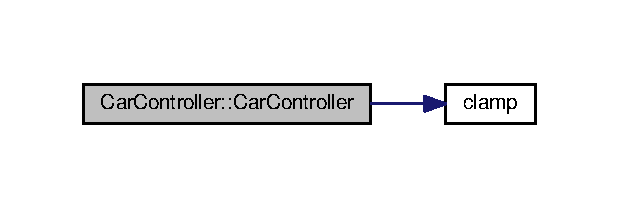
\includegraphics[width=297pt]{class_car_controller_a264969d4b9580b41b7e6d573a18b1de0_cgraph}
\end{center}
\end{figure}




The documentation for this class was generated from the following files\+:\begin{DoxyCompactItemize}
\item 
/home/travis/build/\+Autonomous-\/\+Racing-\/\+P\+G/ros.\+package/docs/master/ros\+\_\+ws/src/car\+\_\+control/include/\hyperlink{car__controller_8h}{car\+\_\+controller.\+h}\item 
/home/travis/build/\+Autonomous-\/\+Racing-\/\+P\+G/ros.\+package/docs/master/ros\+\_\+ws/src/car\+\_\+control/src/\hyperlink{car__controller_8cpp}{car\+\_\+controller.\+cpp}\end{DoxyCompactItemize}

\hypertarget{class_joystick_controller}{}\section{Joystick\+Controller Class Reference}
\label{class_joystick_controller}\index{Joystick\+Controller@{Joystick\+Controller}}


{\ttfamily \#include $<$joystick\+\_\+controller.\+h$>$}

\subsection*{Public Member Functions}
\begin{DoxyCompactItemize}
\item 
\hyperlink{class_joystick_controller_aa7ba7d1b336933c7431ac8796b43c898}{Joystick\+Controller} ()
\begin{DoxyCompactList}\small\item\em Construct a new Remote Joy\+:\+: Remote Joy object. \end{DoxyCompactList}\end{DoxyCompactItemize}


\subsection{Detailed Description}


Definition at line 18 of file joystick\+\_\+controller.\+h.



\subsection{Constructor \& Destructor Documentation}
\index{Joystick\+Controller@{Joystick\+Controller}!Joystick\+Controller@{Joystick\+Controller}}
\index{Joystick\+Controller@{Joystick\+Controller}!Joystick\+Controller@{Joystick\+Controller}}
\subsubsection[{\texorpdfstring{Joystick\+Controller()}{JoystickController()}}]{\setlength{\rightskip}{0pt plus 5cm}Joystick\+Controller\+::\+Joystick\+Controller (
\begin{DoxyParamCaption}
{}
\end{DoxyParamCaption}
)}\hypertarget{class_joystick_controller_aa7ba7d1b336933c7431ac8796b43c898}{}\label{class_joystick_controller_aa7ba7d1b336933c7431ac8796b43c898}


Construct a new Remote Joy\+:\+: Remote Joy object. 



Definition at line 6 of file joystick\+\_\+controller.\+cpp.



The documentation for this class was generated from the following files\+:\begin{DoxyCompactItemize}
\item 
/home/travis/build/\+Autonomous-\/\+Racing-\/\+P\+G/ros.\+package/docs/master/ros\+\_\+ws/src/teleoperation/include/\hyperlink{joystick__controller_8h}{joystick\+\_\+controller.\+h}\item 
/home/travis/build/\+Autonomous-\/\+Racing-\/\+P\+G/ros.\+package/docs/master/ros\+\_\+ws/src/teleoperation/src/\hyperlink{joystick__controller_8cpp}{joystick\+\_\+controller.\+cpp}\end{DoxyCompactItemize}

\hypertarget{class_keyboard_controller}{}\section{Keyboard\+Controller Class Reference}
\label{class_keyboard_controller}\index{Keyboard\+Controller@{Keyboard\+Controller}}


{\ttfamily \#include $<$keyboard\+\_\+controller.\+h$>$}

\subsection*{Public Member Functions}
\begin{DoxyCompactItemize}
\item 
\hyperlink{class_keyboard_controller_abb80b5bae04a1c3cf904924cbacb235c}{Keyboard\+Controller} ()
\item 
\hyperlink{class_keyboard_controller_a102c3356ac118b886b6b5fb7a33245c1}{Keyboard\+Controller} (\hyperlink{class_keyboard_controller}{Keyboard\+Controller} \&\&)=default
\item 
\hyperlink{class_keyboard_controller_a0ea88596f23dbdfa81c80c8c72713957}{Keyboard\+Controller} (const \hyperlink{class_keyboard_controller}{Keyboard\+Controller} \&)=default
\item 
\hyperlink{class_keyboard_controller_a9791aa6d6fadf77b4ef3e59cdb7d9b1d}{$\sim$\+Keyboard\+Controller} ()
\end{DoxyCompactItemize}


\subsection{Detailed Description}


Definition at line 70 of file keyboard\+\_\+controller.\+h.



\subsection{Constructor \& Destructor Documentation}
\index{Keyboard\+Controller@{Keyboard\+Controller}!Keyboard\+Controller@{Keyboard\+Controller}}
\index{Keyboard\+Controller@{Keyboard\+Controller}!Keyboard\+Controller@{Keyboard\+Controller}}
\subsubsection[{\texorpdfstring{Keyboard\+Controller()}{KeyboardController()}}]{\setlength{\rightskip}{0pt plus 5cm}Keyboard\+Controller\+::\+Keyboard\+Controller (
\begin{DoxyParamCaption}
{}
\end{DoxyParamCaption}
)}\hypertarget{class_keyboard_controller_abb80b5bae04a1c3cf904924cbacb235c}{}\label{class_keyboard_controller_abb80b5bae04a1c3cf904924cbacb235c}
Class constructor that sets up a publisher for the drive parameters topic, creates a window and starts a timer for the main loop 

Definition at line 15 of file keyboard\+\_\+controller.\+cpp.

\index{Keyboard\+Controller@{Keyboard\+Controller}!Keyboard\+Controller@{Keyboard\+Controller}}
\index{Keyboard\+Controller@{Keyboard\+Controller}!Keyboard\+Controller@{Keyboard\+Controller}}
\subsubsection[{\texorpdfstring{Keyboard\+Controller(\+Keyboard\+Controller \&\&)=default}{KeyboardController(KeyboardController &&)=default}}]{\setlength{\rightskip}{0pt plus 5cm}Keyboard\+Controller\+::\+Keyboard\+Controller (
\begin{DoxyParamCaption}
\item[{{\bf Keyboard\+Controller} \&\&}]{}
\end{DoxyParamCaption}
)\hspace{0.3cm}{\ttfamily [default]}}\hypertarget{class_keyboard_controller_a102c3356ac118b886b6b5fb7a33245c1}{}\label{class_keyboard_controller_a102c3356ac118b886b6b5fb7a33245c1}
\index{Keyboard\+Controller@{Keyboard\+Controller}!Keyboard\+Controller@{Keyboard\+Controller}}
\index{Keyboard\+Controller@{Keyboard\+Controller}!Keyboard\+Controller@{Keyboard\+Controller}}
\subsubsection[{\texorpdfstring{Keyboard\+Controller(const Keyboard\+Controller \&)=default}{KeyboardController(const KeyboardController &)=default}}]{\setlength{\rightskip}{0pt plus 5cm}Keyboard\+Controller\+::\+Keyboard\+Controller (
\begin{DoxyParamCaption}
\item[{const {\bf Keyboard\+Controller} \&}]{}
\end{DoxyParamCaption}
)\hspace{0.3cm}{\ttfamily [default]}}\hypertarget{class_keyboard_controller_a0ea88596f23dbdfa81c80c8c72713957}{}\label{class_keyboard_controller_a0ea88596f23dbdfa81c80c8c72713957}
\index{Keyboard\+Controller@{Keyboard\+Controller}!````~Keyboard\+Controller@{$\sim$\+Keyboard\+Controller}}
\index{````~Keyboard\+Controller@{$\sim$\+Keyboard\+Controller}!Keyboard\+Controller@{Keyboard\+Controller}}
\subsubsection[{\texorpdfstring{$\sim$\+Keyboard\+Controller()}{~KeyboardController()}}]{\setlength{\rightskip}{0pt plus 5cm}Keyboard\+Controller\+::$\sim$\+Keyboard\+Controller (
\begin{DoxyParamCaption}
{}
\end{DoxyParamCaption}
)}\hypertarget{class_keyboard_controller_a9791aa6d6fadf77b4ef3e59cdb7d9b1d}{}\label{class_keyboard_controller_a9791aa6d6fadf77b4ef3e59cdb7d9b1d}


Definition at line 36 of file keyboard\+\_\+controller.\+cpp.



The documentation for this class was generated from the following files\+:\begin{DoxyCompactItemize}
\item 
/home/travis/build/\+Autonomous-\/\+Racing-\/\+P\+G/ros.\+package/docs/master/ros\+\_\+ws/src/teleoperation/include/\hyperlink{keyboard__controller_8h}{keyboard\+\_\+controller.\+h}\item 
/home/travis/build/\+Autonomous-\/\+Racing-\/\+P\+G/ros.\+package/docs/master/ros\+\_\+ws/src/teleoperation/src/\hyperlink{keyboard__controller_8cpp}{keyboard\+\_\+controller.\+cpp}\end{DoxyCompactItemize}

\chapter{File Documentation}
\hypertarget{mainpage_8dox}{}\section{/home/travis/build/\+Autonomous-\/\+Racing-\/\+P\+G/ros.package/docs/master/doc/mainpage.dox File Reference}
\label{mainpage_8dox}\index{/home/travis/build/\+Autonomous-\/\+Racing-\/\+P\+G/ros.\+package/docs/master/doc/mainpage.\+dox@{/home/travis/build/\+Autonomous-\/\+Racing-\/\+P\+G/ros.\+package/docs/master/doc/mainpage.\+dox}}

\hypertarget{_r_e_a_d_m_e_8md}{}\section{/home/travis/build/\+Autonomous-\/\+Racing-\/\+P\+G/ros.package/\+R\+E\+A\+D\+ME.md File Reference}
\label{_r_e_a_d_m_e_8md}\index{/home/travis/build/\+Autonomous-\/\+Racing-\/\+P\+G/ros.\+package/\+R\+E\+A\+D\+M\+E.\+md@{/home/travis/build/\+Autonomous-\/\+Racing-\/\+P\+G/ros.\+package/\+R\+E\+A\+D\+M\+E.\+md}}

\hypertarget{car__controller_8h}{}\section{/home/travis/build/\+Autonomous-\/\+Racing-\/\+P\+G/ros.package/docs/master/ros\+\_\+ws/src/car\+\_\+control/include/car\+\_\+controller.h File Reference}
\label{car__controller_8h}\index{/home/travis/build/\+Autonomous-\/\+Racing-\/\+P\+G/ros.\+package/docs/master/ros\+\_\+ws/src/car\+\_\+control/include/car\+\_\+controller.\+h@{/home/travis/build/\+Autonomous-\/\+Racing-\/\+P\+G/ros.\+package/docs/master/ros\+\_\+ws/src/car\+\_\+control/include/car\+\_\+controller.\+h}}
{\ttfamily \#include $<$ros/ros.\+h$>$}\\*
{\ttfamily \#include $<$algorithm$>$}\\*
{\ttfamily \#include $<$time.\+h$>$}\\*
{\ttfamily \#include $<$drive\+\_\+msgs/drive\+\_\+param.\+h$>$}\\*
{\ttfamily \#include $<$std\+\_\+msgs/\+Float64.\+h$>$}\\*
{\ttfamily \#include $<$std\+\_\+msgs/\+String.\+h$>$}\\*
Include dependency graph for car\+\_\+controller.\+h\+:
\nopagebreak
\begin{figure}[H]
\begin{center}
\leavevmode
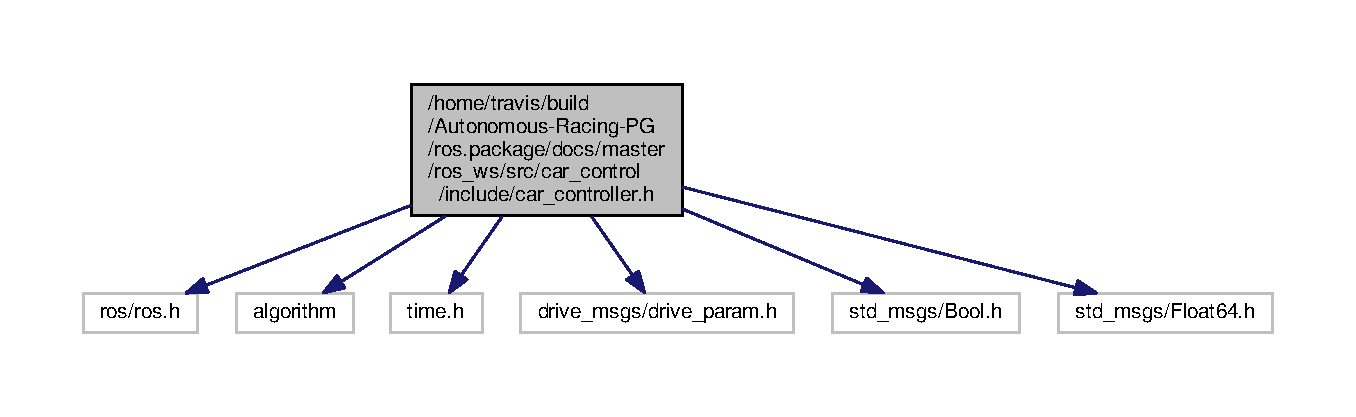
\includegraphics[width=350pt]{car__controller_8h__incl}
\end{center}
\end{figure}
This graph shows which files directly or indirectly include this file\+:
\nopagebreak
\begin{figure}[H]
\begin{center}
\leavevmode
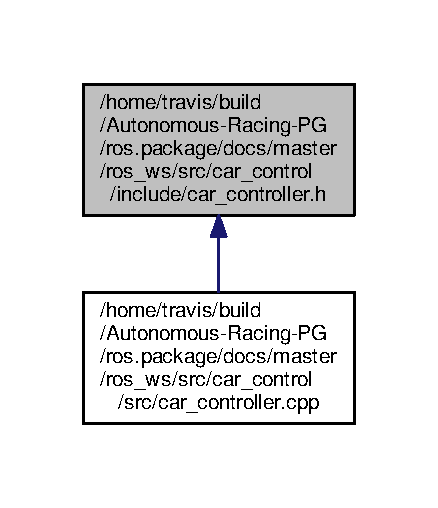
\includegraphics[width=210pt]{car__controller_8h__dep__incl}
\end{center}
\end{figure}
\subsection*{Classes}
\begin{DoxyCompactItemize}
\item 
class \hyperlink{class_car_controller}{Car\+Controller}
\end{DoxyCompactItemize}
\subsection*{Macros}
\begin{DoxyCompactItemize}
\item 
\#define \hyperlink{car__controller_8h_a6977f30ada15874c2885ecd86dab7bd1}{T\+O\+P\+I\+C\+\_\+\+F\+O\+C\+B\+O\+X\+\_\+\+S\+P\+E\+ED}~\char`\"{}/commands/motor/speed\char`\"{}
\item 
\#define \hyperlink{car__controller_8h_a06bf2e121cdcd87f3e73500ff616ccf2}{T\+O\+P\+I\+C\+\_\+\+F\+O\+C\+B\+O\+X\+\_\+\+A\+N\+G\+LE}~\char`\"{}/commands/servo/position\char`\"{}
\item 
\#define \hyperlink{car__controller_8h_a0cad0c0e78519f724d3769a56a6c6412}{T\+O\+P\+I\+C\+\_\+\+D\+R\+I\+V\+E\+\_\+\+P\+A\+R\+AM}~\char`\"{}/set/drive\+\_\+param\char`\"{}
\item 
\#define \hyperlink{car__controller_8h_a23bd7eb4fbfb73461cd96b6fb393c9f5}{T\+O\+P\+I\+C\+\_\+\+C\+O\+M\+M\+A\+ND}~\char`\"{}/command\char`\"{}
\item 
\#define \hyperlink{car__controller_8h_ac2cd96d53dd3ba6407db6766c3d92b26}{M\+A\+X\+\_\+\+S\+P\+E\+ED}~15000
\item 
\#define \hyperlink{car__controller_8h_ad5f5efaa5cb771bd06da4bfe6046809e}{M\+I\+N\+\_\+\+S\+P\+E\+ED}~500
\item 
\#define \hyperlink{car__controller_8h_af3c82099d63a2d91d68bd62d954059c7}{M\+A\+X\+\_\+\+A\+N\+G\+LE}~0.\+9
\end{DoxyCompactItemize}


\subsection{Macro Definition Documentation}
\index{car\+\_\+controller.\+h@{car\+\_\+controller.\+h}!M\+A\+X\+\_\+\+A\+N\+G\+LE@{M\+A\+X\+\_\+\+A\+N\+G\+LE}}
\index{M\+A\+X\+\_\+\+A\+N\+G\+LE@{M\+A\+X\+\_\+\+A\+N\+G\+LE}!car\+\_\+controller.\+h@{car\+\_\+controller.\+h}}
\subsubsection[{\texorpdfstring{M\+A\+X\+\_\+\+A\+N\+G\+LE}{MAX_ANGLE}}]{\setlength{\rightskip}{0pt plus 5cm}\#define M\+A\+X\+\_\+\+A\+N\+G\+LE~0.\+9}\hypertarget{car__controller_8h_af3c82099d63a2d91d68bd62d954059c7}{}\label{car__controller_8h_af3c82099d63a2d91d68bd62d954059c7}


Definition at line 20 of file car\+\_\+controller.\+h.

\index{car\+\_\+controller.\+h@{car\+\_\+controller.\+h}!M\+A\+X\+\_\+\+S\+P\+E\+ED@{M\+A\+X\+\_\+\+S\+P\+E\+ED}}
\index{M\+A\+X\+\_\+\+S\+P\+E\+ED@{M\+A\+X\+\_\+\+S\+P\+E\+ED}!car\+\_\+controller.\+h@{car\+\_\+controller.\+h}}
\subsubsection[{\texorpdfstring{M\+A\+X\+\_\+\+S\+P\+E\+ED}{MAX_SPEED}}]{\setlength{\rightskip}{0pt plus 5cm}\#define M\+A\+X\+\_\+\+S\+P\+E\+ED~15000}\hypertarget{car__controller_8h_ac2cd96d53dd3ba6407db6766c3d92b26}{}\label{car__controller_8h_ac2cd96d53dd3ba6407db6766c3d92b26}


Definition at line 18 of file car\+\_\+controller.\+h.

\index{car\+\_\+controller.\+h@{car\+\_\+controller.\+h}!M\+I\+N\+\_\+\+S\+P\+E\+ED@{M\+I\+N\+\_\+\+S\+P\+E\+ED}}
\index{M\+I\+N\+\_\+\+S\+P\+E\+ED@{M\+I\+N\+\_\+\+S\+P\+E\+ED}!car\+\_\+controller.\+h@{car\+\_\+controller.\+h}}
\subsubsection[{\texorpdfstring{M\+I\+N\+\_\+\+S\+P\+E\+ED}{MIN_SPEED}}]{\setlength{\rightskip}{0pt plus 5cm}\#define M\+I\+N\+\_\+\+S\+P\+E\+ED~500}\hypertarget{car__controller_8h_ad5f5efaa5cb771bd06da4bfe6046809e}{}\label{car__controller_8h_ad5f5efaa5cb771bd06da4bfe6046809e}


Definition at line 19 of file car\+\_\+controller.\+h.

\index{car\+\_\+controller.\+h@{car\+\_\+controller.\+h}!T\+O\+P\+I\+C\+\_\+\+C\+O\+M\+M\+A\+ND@{T\+O\+P\+I\+C\+\_\+\+C\+O\+M\+M\+A\+ND}}
\index{T\+O\+P\+I\+C\+\_\+\+C\+O\+M\+M\+A\+ND@{T\+O\+P\+I\+C\+\_\+\+C\+O\+M\+M\+A\+ND}!car\+\_\+controller.\+h@{car\+\_\+controller.\+h}}
\subsubsection[{\texorpdfstring{T\+O\+P\+I\+C\+\_\+\+C\+O\+M\+M\+A\+ND}{TOPIC_COMMAND}}]{\setlength{\rightskip}{0pt plus 5cm}\#define T\+O\+P\+I\+C\+\_\+\+C\+O\+M\+M\+A\+ND~\char`\"{}/command\char`\"{}}\hypertarget{car__controller_8h_a23bd7eb4fbfb73461cd96b6fb393c9f5}{}\label{car__controller_8h_a23bd7eb4fbfb73461cd96b6fb393c9f5}


Definition at line 16 of file car\+\_\+controller.\+h.

\index{car\+\_\+controller.\+h@{car\+\_\+controller.\+h}!T\+O\+P\+I\+C\+\_\+\+D\+R\+I\+V\+E\+\_\+\+P\+A\+R\+AM@{T\+O\+P\+I\+C\+\_\+\+D\+R\+I\+V\+E\+\_\+\+P\+A\+R\+AM}}
\index{T\+O\+P\+I\+C\+\_\+\+D\+R\+I\+V\+E\+\_\+\+P\+A\+R\+AM@{T\+O\+P\+I\+C\+\_\+\+D\+R\+I\+V\+E\+\_\+\+P\+A\+R\+AM}!car\+\_\+controller.\+h@{car\+\_\+controller.\+h}}
\subsubsection[{\texorpdfstring{T\+O\+P\+I\+C\+\_\+\+D\+R\+I\+V\+E\+\_\+\+P\+A\+R\+AM}{TOPIC_DRIVE_PARAM}}]{\setlength{\rightskip}{0pt plus 5cm}\#define T\+O\+P\+I\+C\+\_\+\+D\+R\+I\+V\+E\+\_\+\+P\+A\+R\+AM~\char`\"{}/set/drive\+\_\+param\char`\"{}}\hypertarget{car__controller_8h_a0cad0c0e78519f724d3769a56a6c6412}{}\label{car__controller_8h_a0cad0c0e78519f724d3769a56a6c6412}


Definition at line 15 of file car\+\_\+controller.\+h.

\index{car\+\_\+controller.\+h@{car\+\_\+controller.\+h}!T\+O\+P\+I\+C\+\_\+\+F\+O\+C\+B\+O\+X\+\_\+\+A\+N\+G\+LE@{T\+O\+P\+I\+C\+\_\+\+F\+O\+C\+B\+O\+X\+\_\+\+A\+N\+G\+LE}}
\index{T\+O\+P\+I\+C\+\_\+\+F\+O\+C\+B\+O\+X\+\_\+\+A\+N\+G\+LE@{T\+O\+P\+I\+C\+\_\+\+F\+O\+C\+B\+O\+X\+\_\+\+A\+N\+G\+LE}!car\+\_\+controller.\+h@{car\+\_\+controller.\+h}}
\subsubsection[{\texorpdfstring{T\+O\+P\+I\+C\+\_\+\+F\+O\+C\+B\+O\+X\+\_\+\+A\+N\+G\+LE}{TOPIC_FOCBOX_ANGLE}}]{\setlength{\rightskip}{0pt plus 5cm}\#define T\+O\+P\+I\+C\+\_\+\+F\+O\+C\+B\+O\+X\+\_\+\+A\+N\+G\+LE~\char`\"{}/commands/servo/position\char`\"{}}\hypertarget{car__controller_8h_a06bf2e121cdcd87f3e73500ff616ccf2}{}\label{car__controller_8h_a06bf2e121cdcd87f3e73500ff616ccf2}


Definition at line 13 of file car\+\_\+controller.\+h.

\index{car\+\_\+controller.\+h@{car\+\_\+controller.\+h}!T\+O\+P\+I\+C\+\_\+\+F\+O\+C\+B\+O\+X\+\_\+\+S\+P\+E\+ED@{T\+O\+P\+I\+C\+\_\+\+F\+O\+C\+B\+O\+X\+\_\+\+S\+P\+E\+ED}}
\index{T\+O\+P\+I\+C\+\_\+\+F\+O\+C\+B\+O\+X\+\_\+\+S\+P\+E\+ED@{T\+O\+P\+I\+C\+\_\+\+F\+O\+C\+B\+O\+X\+\_\+\+S\+P\+E\+ED}!car\+\_\+controller.\+h@{car\+\_\+controller.\+h}}
\subsubsection[{\texorpdfstring{T\+O\+P\+I\+C\+\_\+\+F\+O\+C\+B\+O\+X\+\_\+\+S\+P\+E\+ED}{TOPIC_FOCBOX_SPEED}}]{\setlength{\rightskip}{0pt plus 5cm}\#define T\+O\+P\+I\+C\+\_\+\+F\+O\+C\+B\+O\+X\+\_\+\+S\+P\+E\+ED~\char`\"{}/commands/motor/speed\char`\"{}}\hypertarget{car__controller_8h_a6977f30ada15874c2885ecd86dab7bd1}{}\label{car__controller_8h_a6977f30ada15874c2885ecd86dab7bd1}


Definition at line 12 of file car\+\_\+controller.\+h.


\hypertarget{car__controller_8cpp}{}\section{/home/travis/build/\+Autonomous-\/\+Racing-\/\+P\+G/ros.package/docs/master/ros\+\_\+ws/src/car\+\_\+control/src/car\+\_\+controller.cpp File Reference}
\label{car__controller_8cpp}\index{/home/travis/build/\+Autonomous-\/\+Racing-\/\+P\+G/ros.\+package/docs/master/ros\+\_\+ws/src/car\+\_\+control/src/car\+\_\+controller.\+cpp@{/home/travis/build/\+Autonomous-\/\+Racing-\/\+P\+G/ros.\+package/docs/master/ros\+\_\+ws/src/car\+\_\+control/src/car\+\_\+controller.\+cpp}}
{\ttfamily \#include \char`\"{}car\+\_\+controller.\+h\char`\"{}}\\*
Include dependency graph for car\+\_\+controller.\+cpp\+:
\nopagebreak
\begin{figure}[H]
\begin{center}
\leavevmode
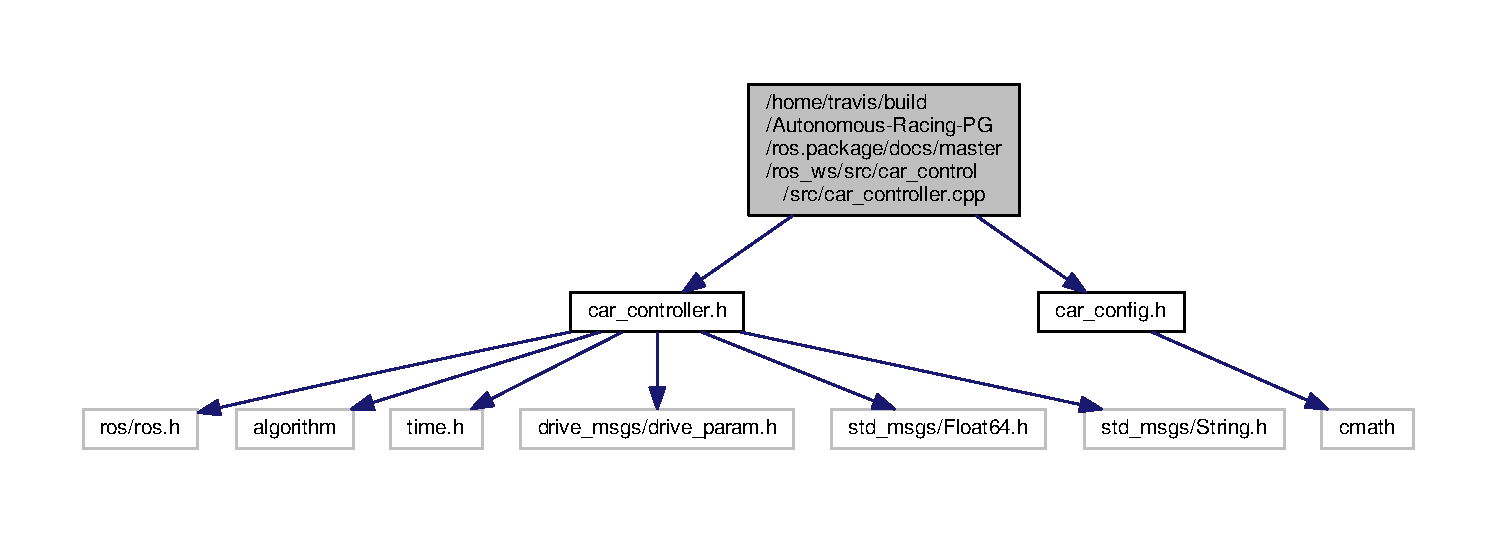
\includegraphics[width=350pt]{car__controller_8cpp__incl}
\end{center}
\end{figure}
\subsection*{Functions}
\begin{DoxyCompactItemize}
\item 
int \hyperlink{car__controller_8cpp_a3c04138a5bfe5d72780bb7e82a18e627}{main} (int argc, char $\ast$$\ast$argv)
\end{DoxyCompactItemize}


\subsection{Function Documentation}
\index{car\+\_\+controller.\+cpp@{car\+\_\+controller.\+cpp}!main@{main}}
\index{main@{main}!car\+\_\+controller.\+cpp@{car\+\_\+controller.\+cpp}}
\subsubsection[{\texorpdfstring{main(int argc, char $\ast$$\ast$argv)}{main(int argc, char **argv)}}]{\setlength{\rightskip}{0pt plus 5cm}int main (
\begin{DoxyParamCaption}
\item[{int}]{argc, }
\item[{char $\ast$$\ast$}]{argv}
\end{DoxyParamCaption}
)}\hypertarget{car__controller_8cpp_a3c04138a5bfe5d72780bb7e82a18e627}{}\label{car__controller_8cpp_a3c04138a5bfe5d72780bb7e82a18e627}


Definition at line 61 of file car\+\_\+controller.\+cpp.


\hypertarget{test__car__control_8cpp}{}\section{/home/travis/build/\+Autonomous-\/\+Racing-\/\+P\+G/ros.package/docs/master/ros\+\_\+ws/src/car\+\_\+control/test/test\+\_\+car\+\_\+control.cpp File Reference}
\label{test__car__control_8cpp}\index{/home/travis/build/\+Autonomous-\/\+Racing-\/\+P\+G/ros.\+package/docs/master/ros\+\_\+ws/src/car\+\_\+control/test/test\+\_\+car\+\_\+control.\+cpp@{/home/travis/build/\+Autonomous-\/\+Racing-\/\+P\+G/ros.\+package/docs/master/ros\+\_\+ws/src/car\+\_\+control/test/test\+\_\+car\+\_\+control.\+cpp}}
{\ttfamily \#include $<$cstdlib$>$}\\*
{\ttfamily \#include $<$gtest/gtest.\+h$>$}\\*
Include dependency graph for test\+\_\+car\+\_\+control.\+cpp\+:
\nopagebreak
\begin{figure}[H]
\begin{center}
\leavevmode
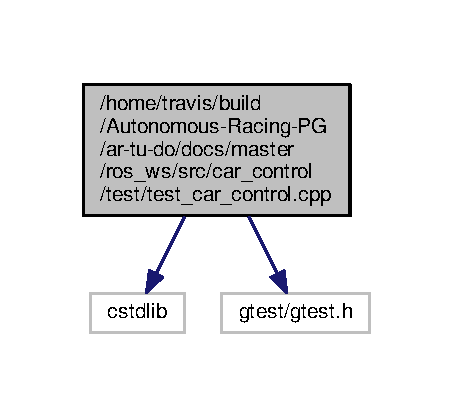
\includegraphics[width=219pt]{test__car__control_8cpp__incl}
\end{center}
\end{figure}
\subsection*{Functions}
\begin{DoxyCompactItemize}
\item 
\hyperlink{test__car__control_8cpp_abdd1a026bf2a8a181d4f4f61169c22f9}{T\+E\+ST} (dummy\+\_\+test, dummy\+\_\+test\+\_\+01)
\item 
\hyperlink{test__car__control_8cpp_a6accdba7cce21b4fbadc9847942eccee}{T\+E\+ST} (dummy\+\_\+test, dummy\+\_\+test\+\_\+02)
\item 
int \hyperlink{test__car__control_8cpp_a3c04138a5bfe5d72780bb7e82a18e627}{main} (int argc, char $\ast$$\ast$argv)
\end{DoxyCompactItemize}


\subsection{Function Documentation}
\index{test\+\_\+car\+\_\+control.\+cpp@{test\+\_\+car\+\_\+control.\+cpp}!main@{main}}
\index{main@{main}!test\+\_\+car\+\_\+control.\+cpp@{test\+\_\+car\+\_\+control.\+cpp}}
\subsubsection[{\texorpdfstring{main(int argc, char $\ast$$\ast$argv)}{main(int argc, char **argv)}}]{\setlength{\rightskip}{0pt plus 5cm}int main (
\begin{DoxyParamCaption}
\item[{int}]{argc, }
\item[{char $\ast$$\ast$}]{argv}
\end{DoxyParamCaption}
)}\hypertarget{test__car__control_8cpp_a3c04138a5bfe5d72780bb7e82a18e627}{}\label{test__car__control_8cpp_a3c04138a5bfe5d72780bb7e82a18e627}


Definition at line 20 of file test\+\_\+car\+\_\+control.\+cpp.

\index{test\+\_\+car\+\_\+control.\+cpp@{test\+\_\+car\+\_\+control.\+cpp}!T\+E\+ST@{T\+E\+ST}}
\index{T\+E\+ST@{T\+E\+ST}!test\+\_\+car\+\_\+control.\+cpp@{test\+\_\+car\+\_\+control.\+cpp}}
\subsubsection[{\texorpdfstring{T\+E\+S\+T(dummy\+\_\+test, dummy\+\_\+test\+\_\+01)}{TEST(dummy_test, dummy_test_01)}}]{\setlength{\rightskip}{0pt plus 5cm}T\+E\+ST (
\begin{DoxyParamCaption}
\item[{dummy\+\_\+test}]{, }
\item[{dummy\+\_\+test\+\_\+01}]{}
\end{DoxyParamCaption}
)}\hypertarget{test__car__control_8cpp_abdd1a026bf2a8a181d4f4f61169c22f9}{}\label{test__car__control_8cpp_abdd1a026bf2a8a181d4f4f61169c22f9}


Definition at line 10 of file test\+\_\+car\+\_\+control.\+cpp.

\index{test\+\_\+car\+\_\+control.\+cpp@{test\+\_\+car\+\_\+control.\+cpp}!T\+E\+ST@{T\+E\+ST}}
\index{T\+E\+ST@{T\+E\+ST}!test\+\_\+car\+\_\+control.\+cpp@{test\+\_\+car\+\_\+control.\+cpp}}
\subsubsection[{\texorpdfstring{T\+E\+S\+T(dummy\+\_\+test, dummy\+\_\+test\+\_\+02)}{TEST(dummy_test, dummy_test_02)}}]{\setlength{\rightskip}{0pt plus 5cm}T\+E\+ST (
\begin{DoxyParamCaption}
\item[{dummy\+\_\+test}]{, }
\item[{dummy\+\_\+test\+\_\+02}]{}
\end{DoxyParamCaption}
)}\hypertarget{test__car__control_8cpp_a6accdba7cce21b4fbadc9847942eccee}{}\label{test__car__control_8cpp_a6accdba7cce21b4fbadc9847942eccee}


Definition at line 15 of file test\+\_\+car\+\_\+control.\+cpp.


\hypertarget{drive__param__converter_8py}{}\section{/home/travis/build/\+Autonomous-\/\+Racing-\/\+P\+G/ros.package/docs/master/ros\+\_\+ws/src/simulation/racer\+\_\+control/scripts/drive\+\_\+param\+\_\+converter.py File Reference}
\label{drive__param__converter_8py}\index{/home/travis/build/\+Autonomous-\/\+Racing-\/\+P\+G/ros.\+package/docs/master/ros\+\_\+ws/src/simulation/racer\+\_\+control/scripts/drive\+\_\+param\+\_\+converter.\+py@{/home/travis/build/\+Autonomous-\/\+Racing-\/\+P\+G/ros.\+package/docs/master/ros\+\_\+ws/src/simulation/racer\+\_\+control/scripts/drive\+\_\+param\+\_\+converter.\+py}}
\subsection*{Namespaces}
\begin{DoxyCompactItemize}
\item 
 \hyperlink{namespacedrive__param__converter}{drive\+\_\+param\+\_\+converter}
\end{DoxyCompactItemize}
\subsection*{Functions}
\begin{DoxyCompactItemize}
\item 
def \hyperlink{namespacedrive__param__converter_afdd5fa91c648e8545fae1cd833995f40}{drive\+\_\+param\+\_\+converter.\+set\+\_\+throttle\+\_\+steer} (data)
\item 
def \hyperlink{namespacedrive__param__converter_a14d9041f6f5fd041bfbea4f26cbe0155}{drive\+\_\+param\+\_\+converter.\+drive\+\_\+param\+\_\+converter} ()
\end{DoxyCompactItemize}
\subsection*{Variables}
\begin{DoxyCompactItemize}
\item 
int \hyperlink{namespacedrive__param__converter_aab4bf01f556d80bbeeb22edf8bf07611}{drive\+\_\+param\+\_\+converter.\+flag\+\_\+move} = 0
\end{DoxyCompactItemize}

\hypertarget{joystick__controller_8h}{}\section{/home/travis/build/\+Autonomous-\/\+Racing-\/\+P\+G/ros.package/docs/master/ros\+\_\+ws/src/teleoperation/include/joystick\+\_\+controller.h File Reference}
\label{joystick__controller_8h}\index{/home/travis/build/\+Autonomous-\/\+Racing-\/\+P\+G/ros.\+package/docs/master/ros\+\_\+ws/src/teleoperation/include/joystick\+\_\+controller.\+h@{/home/travis/build/\+Autonomous-\/\+Racing-\/\+P\+G/ros.\+package/docs/master/ros\+\_\+ws/src/teleoperation/include/joystick\+\_\+controller.\+h}}
{\ttfamily \#include $<$ros/ros.\+h$>$}\\*
{\ttfamily \#include $<$chrono$>$}\\*
{\ttfamily \#include $<$drive\+\_\+msgs/drive\+\_\+param.\+h$>$}\\*
{\ttfamily \#include $<$sensor\+\_\+msgs/\+Joy.\+h$>$}\\*
{\ttfamily \#include $<$string$>$}\\*
Include dependency graph for joystick\+\_\+controller.\+h\+:
\nopagebreak
\begin{figure}[H]
\begin{center}
\leavevmode
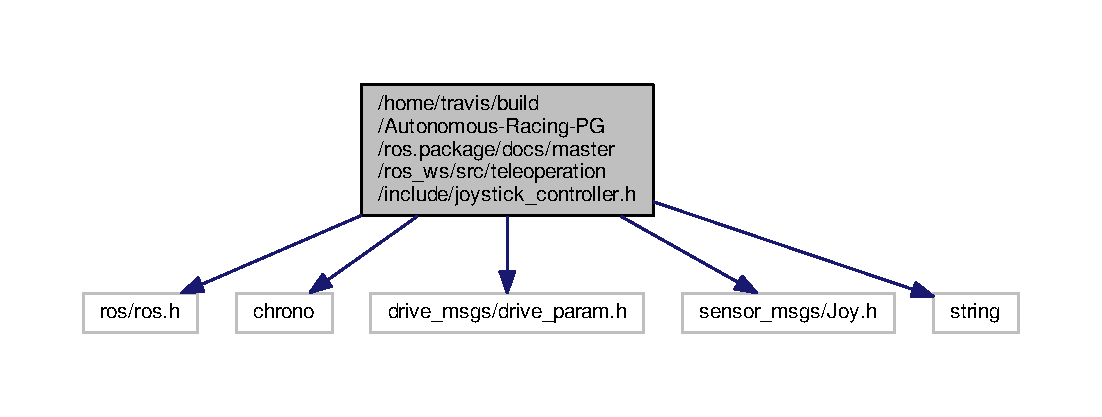
\includegraphics[width=350pt]{joystick__controller_8h__incl}
\end{center}
\end{figure}
This graph shows which files directly or indirectly include this file\+:
\nopagebreak
\begin{figure}[H]
\begin{center}
\leavevmode
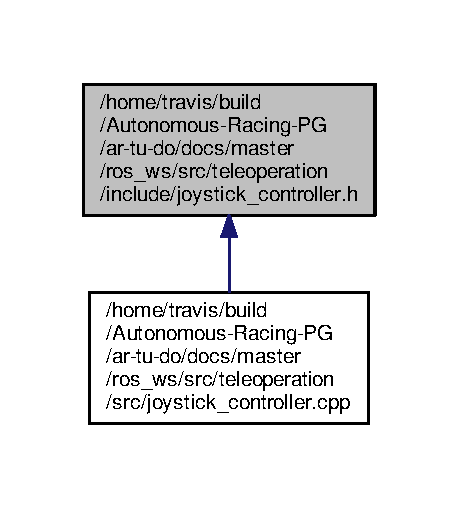
\includegraphics[width=220pt]{joystick__controller_8h__dep__incl}
\end{center}
\end{figure}
\subsection*{Classes}
\begin{DoxyCompactItemize}
\item 
class \hyperlink{class_joystick_controller}{Joystick\+Controller}
\end{DoxyCompactItemize}
\subsection*{Variables}
\begin{DoxyCompactItemize}
\item 
constexpr const char $\ast$ \hyperlink{joystick__controller_8h_ab1fc9856ff20e19b2de5cec9f118a527}{P\+A\+R\+A\+M\+E\+T\+E\+R\+\_\+\+J\+O\+Y\+S\+T\+I\+C\+K\+\_\+\+T\+Y\+PE} = \char`\"{}joystick\+\_\+type\char`\"{}
\item 
constexpr const char $\ast$ \hyperlink{joystick__controller_8h_a3881a7dd470107a7c50efedc0a708839}{T\+O\+P\+I\+C\+\_\+\+D\+R\+I\+V\+E\+\_\+\+P\+A\+R\+A\+M\+E\+T\+E\+RS} = \char`\"{}input/drive\+\_\+param/joystick\char`\"{}
\item 
constexpr const char $\ast$ \hyperlink{joystick__controller_8h_a1e56417499d1048f130bc194015c7bef}{T\+O\+P\+I\+C\+\_\+\+D\+MS} = \char`\"{}/set/dms\char`\"{}
\item 
constexpr float \hyperlink{joystick__controller_8h_ae0a6c00cd55e4ce8887e55979ac45f75}{A\+C\+C\+E\+L\+E\+R\+A\+T\+I\+O\+N\+\_\+\+S\+C\+A\+L\+I\+N\+G\+\_\+\+F\+A\+C\+T\+OR} = 0.\+1f
\begin{DoxyCompactList}\small\item\em scales the absolute acceleration provided by the joystick. Useful if the car should not drive with 100\% speed if acceleration button is fully pressed \end{DoxyCompactList}\item 
constexpr float \hyperlink{joystick__controller_8h_a27923d1c16e61de371e62e7aff73147e}{D\+E\+C\+E\+L\+E\+R\+A\+T\+I\+O\+N\+\_\+\+S\+C\+A\+L\+I\+N\+G\+\_\+\+F\+A\+C\+T\+OR} = 0.\+1f
\begin{DoxyCompactList}\small\item\em scales the absolute deceleration provided by the joystick. Useful if the car should not decelerate with 100\% speed if deceleration button is fully pressed \end{DoxyCompactList}\item 
constexpr float \hyperlink{joystick__controller_8h_a55c5df50bc18dcffbb973707048fca39}{S\+T\+E\+E\+R\+I\+N\+G\+\_\+\+S\+C\+A\+L\+I\+N\+G\+\_\+\+F\+A\+C\+T\+OR} = 0.\+8f
\begin{DoxyCompactList}\small\item\em scales the absolute steering value (between -\/1 and 1) provided by the joystick. Useful if the car should not steer 100\% left and right \end{DoxyCompactList}\end{DoxyCompactItemize}


\subsection{Variable Documentation}
\index{joystick\+\_\+controller.\+h@{joystick\+\_\+controller.\+h}!A\+C\+C\+E\+L\+E\+R\+A\+T\+I\+O\+N\+\_\+\+S\+C\+A\+L\+I\+N\+G\+\_\+\+F\+A\+C\+T\+OR@{A\+C\+C\+E\+L\+E\+R\+A\+T\+I\+O\+N\+\_\+\+S\+C\+A\+L\+I\+N\+G\+\_\+\+F\+A\+C\+T\+OR}}
\index{A\+C\+C\+E\+L\+E\+R\+A\+T\+I\+O\+N\+\_\+\+S\+C\+A\+L\+I\+N\+G\+\_\+\+F\+A\+C\+T\+OR@{A\+C\+C\+E\+L\+E\+R\+A\+T\+I\+O\+N\+\_\+\+S\+C\+A\+L\+I\+N\+G\+\_\+\+F\+A\+C\+T\+OR}!joystick\+\_\+controller.\+h@{joystick\+\_\+controller.\+h}}
\subsubsection[{\texorpdfstring{A\+C\+C\+E\+L\+E\+R\+A\+T\+I\+O\+N\+\_\+\+S\+C\+A\+L\+I\+N\+G\+\_\+\+F\+A\+C\+T\+OR}{ACCELERATION_SCALING_FACTOR}}]{\setlength{\rightskip}{0pt plus 5cm}constexpr float A\+C\+C\+E\+L\+E\+R\+A\+T\+I\+O\+N\+\_\+\+S\+C\+A\+L\+I\+N\+G\+\_\+\+F\+A\+C\+T\+OR = 0.\+1f}\hypertarget{joystick__controller_8h_ae0a6c00cd55e4ce8887e55979ac45f75}{}\label{joystick__controller_8h_ae0a6c00cd55e4ce8887e55979ac45f75}


scales the absolute acceleration provided by the joystick. Useful if the car should not drive with 100\% speed if acceleration button is fully pressed 



Definition at line 18 of file joystick\+\_\+controller.\+h.

\index{joystick\+\_\+controller.\+h@{joystick\+\_\+controller.\+h}!D\+E\+C\+E\+L\+E\+R\+A\+T\+I\+O\+N\+\_\+\+S\+C\+A\+L\+I\+N\+G\+\_\+\+F\+A\+C\+T\+OR@{D\+E\+C\+E\+L\+E\+R\+A\+T\+I\+O\+N\+\_\+\+S\+C\+A\+L\+I\+N\+G\+\_\+\+F\+A\+C\+T\+OR}}
\index{D\+E\+C\+E\+L\+E\+R\+A\+T\+I\+O\+N\+\_\+\+S\+C\+A\+L\+I\+N\+G\+\_\+\+F\+A\+C\+T\+OR@{D\+E\+C\+E\+L\+E\+R\+A\+T\+I\+O\+N\+\_\+\+S\+C\+A\+L\+I\+N\+G\+\_\+\+F\+A\+C\+T\+OR}!joystick\+\_\+controller.\+h@{joystick\+\_\+controller.\+h}}
\subsubsection[{\texorpdfstring{D\+E\+C\+E\+L\+E\+R\+A\+T\+I\+O\+N\+\_\+\+S\+C\+A\+L\+I\+N\+G\+\_\+\+F\+A\+C\+T\+OR}{DECELERATION_SCALING_FACTOR}}]{\setlength{\rightskip}{0pt plus 5cm}constexpr float D\+E\+C\+E\+L\+E\+R\+A\+T\+I\+O\+N\+\_\+\+S\+C\+A\+L\+I\+N\+G\+\_\+\+F\+A\+C\+T\+OR = 0.\+1f}\hypertarget{joystick__controller_8h_a27923d1c16e61de371e62e7aff73147e}{}\label{joystick__controller_8h_a27923d1c16e61de371e62e7aff73147e}


scales the absolute deceleration provided by the joystick. Useful if the car should not decelerate with 100\% speed if deceleration button is fully pressed 



Definition at line 24 of file joystick\+\_\+controller.\+h.

\index{joystick\+\_\+controller.\+h@{joystick\+\_\+controller.\+h}!P\+A\+R\+A\+M\+E\+T\+E\+R\+\_\+\+J\+O\+Y\+S\+T\+I\+C\+K\+\_\+\+T\+Y\+PE@{P\+A\+R\+A\+M\+E\+T\+E\+R\+\_\+\+J\+O\+Y\+S\+T\+I\+C\+K\+\_\+\+T\+Y\+PE}}
\index{P\+A\+R\+A\+M\+E\+T\+E\+R\+\_\+\+J\+O\+Y\+S\+T\+I\+C\+K\+\_\+\+T\+Y\+PE@{P\+A\+R\+A\+M\+E\+T\+E\+R\+\_\+\+J\+O\+Y\+S\+T\+I\+C\+K\+\_\+\+T\+Y\+PE}!joystick\+\_\+controller.\+h@{joystick\+\_\+controller.\+h}}
\subsubsection[{\texorpdfstring{P\+A\+R\+A\+M\+E\+T\+E\+R\+\_\+\+J\+O\+Y\+S\+T\+I\+C\+K\+\_\+\+T\+Y\+PE}{PARAMETER_JOYSTICK_TYPE}}]{\setlength{\rightskip}{0pt plus 5cm}constexpr const char$\ast$ P\+A\+R\+A\+M\+E\+T\+E\+R\+\_\+\+J\+O\+Y\+S\+T\+I\+C\+K\+\_\+\+T\+Y\+PE = \char`\"{}joystick\+\_\+type\char`\"{}}\hypertarget{joystick__controller_8h_ab1fc9856ff20e19b2de5cec9f118a527}{}\label{joystick__controller_8h_ab1fc9856ff20e19b2de5cec9f118a527}


Definition at line 10 of file joystick\+\_\+controller.\+h.

\index{joystick\+\_\+controller.\+h@{joystick\+\_\+controller.\+h}!S\+T\+E\+E\+R\+I\+N\+G\+\_\+\+S\+C\+A\+L\+I\+N\+G\+\_\+\+F\+A\+C\+T\+OR@{S\+T\+E\+E\+R\+I\+N\+G\+\_\+\+S\+C\+A\+L\+I\+N\+G\+\_\+\+F\+A\+C\+T\+OR}}
\index{S\+T\+E\+E\+R\+I\+N\+G\+\_\+\+S\+C\+A\+L\+I\+N\+G\+\_\+\+F\+A\+C\+T\+OR@{S\+T\+E\+E\+R\+I\+N\+G\+\_\+\+S\+C\+A\+L\+I\+N\+G\+\_\+\+F\+A\+C\+T\+OR}!joystick\+\_\+controller.\+h@{joystick\+\_\+controller.\+h}}
\subsubsection[{\texorpdfstring{S\+T\+E\+E\+R\+I\+N\+G\+\_\+\+S\+C\+A\+L\+I\+N\+G\+\_\+\+F\+A\+C\+T\+OR}{STEERING_SCALING_FACTOR}}]{\setlength{\rightskip}{0pt plus 5cm}constexpr float S\+T\+E\+E\+R\+I\+N\+G\+\_\+\+S\+C\+A\+L\+I\+N\+G\+\_\+\+F\+A\+C\+T\+OR = 0.\+8f}\hypertarget{joystick__controller_8h_a55c5df50bc18dcffbb973707048fca39}{}\label{joystick__controller_8h_a55c5df50bc18dcffbb973707048fca39}


scales the absolute steering value (between -\/1 and 1) provided by the joystick. Useful if the car should not steer 100\% left and right 



Definition at line 30 of file joystick\+\_\+controller.\+h.

\index{joystick\+\_\+controller.\+h@{joystick\+\_\+controller.\+h}!T\+O\+P\+I\+C\+\_\+\+D\+MS@{T\+O\+P\+I\+C\+\_\+\+D\+MS}}
\index{T\+O\+P\+I\+C\+\_\+\+D\+MS@{T\+O\+P\+I\+C\+\_\+\+D\+MS}!joystick\+\_\+controller.\+h@{joystick\+\_\+controller.\+h}}
\subsubsection[{\texorpdfstring{T\+O\+P\+I\+C\+\_\+\+D\+MS}{TOPIC_DMS}}]{\setlength{\rightskip}{0pt plus 5cm}constexpr const char$\ast$ T\+O\+P\+I\+C\+\_\+\+D\+MS = \char`\"{}/set/dms\char`\"{}}\hypertarget{joystick__controller_8h_a1e56417499d1048f130bc194015c7bef}{}\label{joystick__controller_8h_a1e56417499d1048f130bc194015c7bef}


Definition at line 12 of file joystick\+\_\+controller.\+h.

\index{joystick\+\_\+controller.\+h@{joystick\+\_\+controller.\+h}!T\+O\+P\+I\+C\+\_\+\+D\+R\+I\+V\+E\+\_\+\+P\+A\+R\+A\+M\+E\+T\+E\+RS@{T\+O\+P\+I\+C\+\_\+\+D\+R\+I\+V\+E\+\_\+\+P\+A\+R\+A\+M\+E\+T\+E\+RS}}
\index{T\+O\+P\+I\+C\+\_\+\+D\+R\+I\+V\+E\+\_\+\+P\+A\+R\+A\+M\+E\+T\+E\+RS@{T\+O\+P\+I\+C\+\_\+\+D\+R\+I\+V\+E\+\_\+\+P\+A\+R\+A\+M\+E\+T\+E\+RS}!joystick\+\_\+controller.\+h@{joystick\+\_\+controller.\+h}}
\subsubsection[{\texorpdfstring{T\+O\+P\+I\+C\+\_\+\+D\+R\+I\+V\+E\+\_\+\+P\+A\+R\+A\+M\+E\+T\+E\+RS}{TOPIC_DRIVE_PARAMETERS}}]{\setlength{\rightskip}{0pt plus 5cm}constexpr const char$\ast$ T\+O\+P\+I\+C\+\_\+\+D\+R\+I\+V\+E\+\_\+\+P\+A\+R\+A\+M\+E\+T\+E\+RS = \char`\"{}input/drive\+\_\+param/joystick\char`\"{}}\hypertarget{joystick__controller_8h_a3881a7dd470107a7c50efedc0a708839}{}\label{joystick__controller_8h_a3881a7dd470107a7c50efedc0a708839}


Definition at line 11 of file joystick\+\_\+controller.\+h.


\hypertarget{keyboard__controller_8h}{}\section{/home/travis/build/\+Autonomous-\/\+Racing-\/\+P\+G/ros.package/docs/master/ros\+\_\+ws/src/teleoperation/include/keyboard\+\_\+controller.h File Reference}
\label{keyboard__controller_8h}\index{/home/travis/build/\+Autonomous-\/\+Racing-\/\+P\+G/ros.\+package/docs/master/ros\+\_\+ws/src/teleoperation/include/keyboard\+\_\+controller.\+h@{/home/travis/build/\+Autonomous-\/\+Racing-\/\+P\+G/ros.\+package/docs/master/ros\+\_\+ws/src/teleoperation/include/keyboard\+\_\+controller.\+h}}
{\ttfamily \#include $<$S\+D\+L2/\+S\+D\+L.\+h$>$}\\*
{\ttfamily \#include $<$algorithm$>$}\\*
{\ttfamily \#include $<$array$>$}\\*
{\ttfamily \#include $<$drive\+\_\+msgs/drive\+\_\+param.\+h$>$}\\*
{\ttfamily \#include $<$ros/package.\+h$>$}\\*
{\ttfamily \#include $<$ros/ros.\+h$>$}\\*
{\ttfamily \#include $<$signal.\+h$>$}\\*
{\ttfamily \#include $<$std\+\_\+msgs/\+String.\+h$>$}\\*
{\ttfamily \#include $<$stdexcept$>$}\\*
Include dependency graph for keyboard\+\_\+controller.\+h\+:
\nopagebreak
\begin{figure}[H]
\begin{center}
\leavevmode
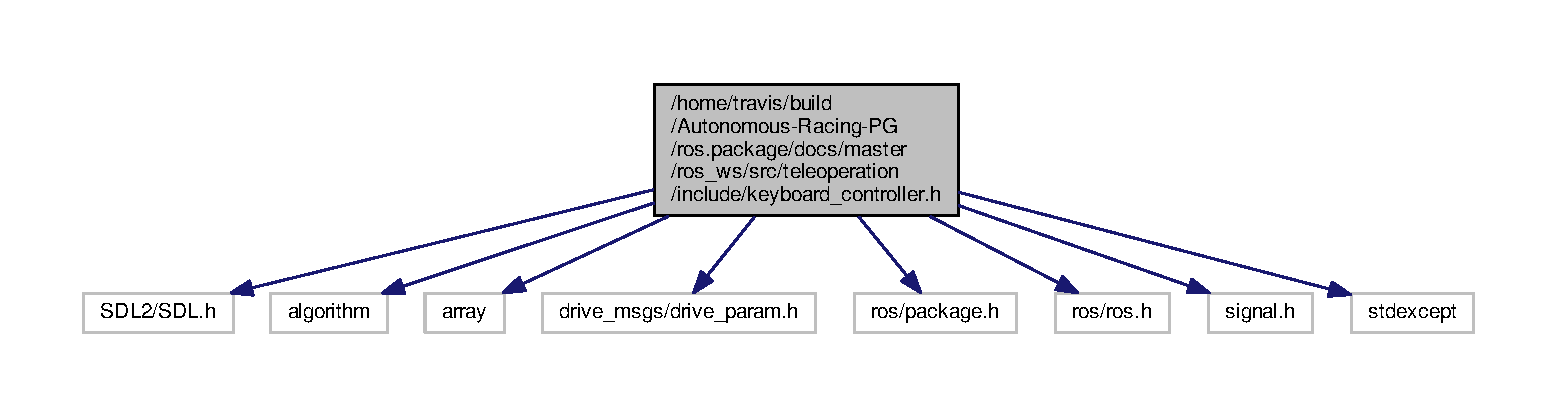
\includegraphics[width=350pt]{keyboard__controller_8h__incl}
\end{center}
\end{figure}
This graph shows which files directly or indirectly include this file\+:
\nopagebreak
\begin{figure}[H]
\begin{center}
\leavevmode
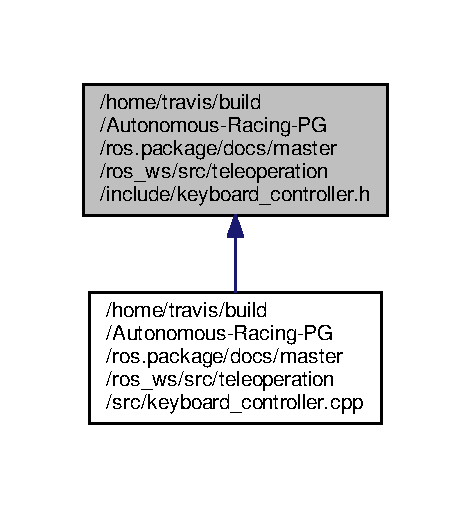
\includegraphics[width=226pt]{keyboard__controller_8h__dep__incl}
\end{center}
\end{figure}
\subsection*{Classes}
\begin{DoxyCompactItemize}
\item 
class \hyperlink{class_keyboard_controller}{Keyboard\+Controller}
\end{DoxyCompactItemize}
\subsection*{Enumerations}
\begin{DoxyCompactItemize}
\item 
enum \hyperlink{keyboard__controller_8h_a28fdc629dbeaa30236718d9093e19c07}{Keycode} \+: int \{ \\*
\hyperlink{keyboard__controller_8h_a28fdc629dbeaa30236718d9093e19c07a61e9c06ea9a85a5088a499df6458d276}{Keycode\+::W} = 119, 
\hyperlink{keyboard__controller_8h_a28fdc629dbeaa30236718d9093e19c07a7fc56270e7a70fa81a5935b72eacbe29}{Keycode\+::A} = 97, 
\hyperlink{keyboard__controller_8h_a28fdc629dbeaa30236718d9093e19c07a5dbc98dcc983a70728bd082d1a47546e}{Keycode\+::S} = 115, 
\hyperlink{keyboard__controller_8h_a28fdc629dbeaa30236718d9093e19c07af623e75af30e62bbd73d6df5b50bb7b5}{Keycode\+::D} = 100, 
\\*
\hyperlink{keyboard__controller_8h_a28fdc629dbeaa30236718d9093e19c07a6506ae39fdca9845e3a6de3865183e57}{Keycode\+::\+S\+P\+A\+CE} = 32
 \}
\item 
enum \hyperlink{keyboard__controller_8h_a4f3852c29660b2c7415360633c54e0bb}{Key\+Index} \+: int \{ \\*
\hyperlink{keyboard__controller_8h_a4f3852c29660b2c7415360633c54e0bbae8637671ccf72cd596fe0c2d1af5ad20}{Key\+Index\+::\+A\+C\+C\+E\+L\+E\+R\+A\+TE} = 0, 
\hyperlink{keyboard__controller_8h_a4f3852c29660b2c7415360633c54e0bbaceeff3cb59294b233b481ddb6dee95bf}{Key\+Index\+::\+D\+E\+C\+E\+L\+E\+R\+A\+TE} = 2, 
\hyperlink{keyboard__controller_8h_a4f3852c29660b2c7415360633c54e0bbace64911e4c5738134f296b7e7706fd86}{Key\+Index\+::\+S\+T\+E\+E\+R\+\_\+\+L\+E\+FT} = 1, 
\hyperlink{keyboard__controller_8h_a4f3852c29660b2c7415360633c54e0bba2f519bbf001708f1709b0b01550e76d9}{Key\+Index\+::\+S\+T\+E\+E\+R\+\_\+\+R\+I\+G\+HT} = 3, 
\\*
\hyperlink{keyboard__controller_8h_a4f3852c29660b2c7415360633c54e0bba5ea9ff88324a0fcc230686e273a00de1}{Key\+Index\+::\+D\+E\+A\+D\+\_\+\+M\+A\+N\+S\+\_\+\+S\+W\+I\+T\+CH} = 4
 \}
\end{DoxyCompactItemize}
\subsection*{Variables}
\begin{DoxyCompactItemize}
\item 
constexpr const char $\ast$ \hyperlink{keyboard__controller_8h_a3881a7dd470107a7c50efedc0a708839}{T\+O\+P\+I\+C\+\_\+\+D\+R\+I\+V\+E\+\_\+\+P\+A\+R\+A\+M\+E\+T\+E\+RS} = \char`\"{}/set/drive\+\_\+param\char`\"{}
\item 
constexpr const char $\ast$ \hyperlink{keyboard__controller_8h_aabd38024f2f1a3ffba466bdd55e1142c}{T\+O\+P\+I\+C\+\_\+\+D\+E\+A\+D\+\_\+\+M\+A\+N\+S\+\_\+\+S\+W\+I\+T\+CH} = \char`\"{}/set/dms\char`\"{}
\item 
constexpr const char $\ast$ \hyperlink{keyboard__controller_8h_a0f7f9cc9b6a6ff34aaf9f7acd8d3d044}{T\+O\+P\+I\+C\+\_\+\+C\+O\+M\+M\+A\+ND} = \char`\"{}/command\char`\"{}
\item 
constexpr const char $\ast$ \hyperlink{keyboard__controller_8h_a6d4b6e4b84736143609cad22046a82fa}{C\+O\+M\+M\+A\+N\+D\+\_\+\+S\+T\+OP} = \char`\"{}stop\char`\"{}
\item 
constexpr const char $\ast$ \hyperlink{keyboard__controller_8h_a3ba962d8165c56ab8545410f4edd510f}{C\+O\+M\+M\+A\+N\+D\+\_\+\+GO} = \char`\"{}go\char`\"{}
\item 
constexpr int \hyperlink{keyboard__controller_8h_a19ecc164327668cf4b24f872053a3dd5}{K\+E\+Y\+\_\+\+C\+O\+U\+NT} = 5
\item 
constexpr std\+::array$<$ \hyperlink{keyboard__controller_8h_a28fdc629dbeaa30236718d9093e19c07}{Keycode}, \hyperlink{keyboard__controller_8h_a19ecc164327668cf4b24f872053a3dd5}{K\+E\+Y\+\_\+\+C\+O\+U\+NT} $>$ \hyperlink{keyboard__controller_8h_a2c20c56647297ef05c4808bbb77b05dc}{K\+E\+Y\+\_\+\+C\+O\+D\+ES} = \{ \hyperlink{keyboard__controller_8h_a28fdc629dbeaa30236718d9093e19c07a61e9c06ea9a85a5088a499df6458d276}{Keycode\+::W}, \hyperlink{keyboard__controller_8h_a28fdc629dbeaa30236718d9093e19c07a7fc56270e7a70fa81a5935b72eacbe29}{Keycode\+::A}, \hyperlink{keyboard__controller_8h_a28fdc629dbeaa30236718d9093e19c07a5dbc98dcc983a70728bd082d1a47546e}{Keycode\+::S}, \hyperlink{keyboard__controller_8h_a28fdc629dbeaa30236718d9093e19c07af623e75af30e62bbd73d6df5b50bb7b5}{Keycode\+::D}, \hyperlink{keyboard__controller_8h_a28fdc629dbeaa30236718d9093e19c07a6506ae39fdca9845e3a6de3865183e57}{Keycode\+::\+S\+P\+A\+CE} \}
\item 
constexpr double \hyperlink{keyboard__controller_8h_a87d3197843880cb61cbecb5379db066c}{P\+A\+R\+A\+M\+E\+T\+E\+R\+\_\+\+U\+P\+D\+A\+T\+E\+\_\+\+F\+R\+E\+Q\+U\+E\+N\+CY} = 90
\item 
constexpr double \hyperlink{keyboard__controller_8h_ad9063d7d546c70bfc9b5f9d575b594c5}{S\+T\+E\+E\+R\+I\+N\+G\+\_\+\+S\+P\+E\+ED} = 6
\item 
constexpr double \hyperlink{keyboard__controller_8h_a7f06f2775e2c7469140a29018ae10261}{A\+C\+C\+E\+L\+E\+R\+A\+T\+I\+ON} = 0.\+4
\item 
constexpr double \hyperlink{keyboard__controller_8h_ae3d69992cbd260ed0f86a4e5fd735d4e}{B\+R\+A\+K\+I\+NG} = 2
\item 
constexpr double \hyperlink{keyboard__controller_8h_a615bf3b38c23cb483977c1943449ce87}{F\+A\+S\+T\+\_\+\+S\+T\+E\+E\+R\+\_\+\+L\+I\+M\+IT} = 0.\+6
\item 
constexpr double \hyperlink{keyboard__controller_8h_a8cfb8f83cd91665c0b18f3e213edf672}{S\+T\+E\+E\+R\+I\+N\+G\+\_\+\+G\+R\+A\+V\+I\+TY} = 2
\item 
constexpr double \hyperlink{keyboard__controller_8h_ac0e74cb464c171072d0130141d519a3b}{T\+H\+R\+O\+T\+T\+L\+E\+\_\+\+G\+R\+A\+V\+I\+TY} = 3
\item 
constexpr double \hyperlink{keyboard__controller_8h_a670fdc7f227b3ed454e9e4b01d9bf117}{M\+A\+X\+\_\+\+T\+H\+R\+O\+T\+T\+LE} = 0.\+25
\end{DoxyCompactItemize}


\subsection{Enumeration Type Documentation}
\index{keyboard\+\_\+controller.\+h@{keyboard\+\_\+controller.\+h}!Keycode@{Keycode}}
\index{Keycode@{Keycode}!keyboard\+\_\+controller.\+h@{keyboard\+\_\+controller.\+h}}
\subsubsection[{\texorpdfstring{Keycode}{Keycode}}]{\setlength{\rightskip}{0pt plus 5cm}enum {\bf Keycode} \+: int\hspace{0.3cm}{\ttfamily [strong]}}\hypertarget{keyboard__controller_8h_a28fdc629dbeaa30236718d9093e19c07}{}\label{keyboard__controller_8h_a28fdc629dbeaa30236718d9093e19c07}
\begin{Desc}
\item[Enumerator]\par
\begin{description}
\index{W@{W}!keyboard\+\_\+controller.\+h@{keyboard\+\_\+controller.\+h}}\index{keyboard\+\_\+controller.\+h@{keyboard\+\_\+controller.\+h}!W@{W}}\item[{\em 
W\hypertarget{keyboard__controller_8h_a28fdc629dbeaa30236718d9093e19c07a61e9c06ea9a85a5088a499df6458d276}{}\label{keyboard__controller_8h_a28fdc629dbeaa30236718d9093e19c07a61e9c06ea9a85a5088a499df6458d276}
}]\index{A@{A}!keyboard\+\_\+controller.\+h@{keyboard\+\_\+controller.\+h}}\index{keyboard\+\_\+controller.\+h@{keyboard\+\_\+controller.\+h}!A@{A}}\item[{\em 
A\hypertarget{keyboard__controller_8h_a28fdc629dbeaa30236718d9093e19c07a7fc56270e7a70fa81a5935b72eacbe29}{}\label{keyboard__controller_8h_a28fdc629dbeaa30236718d9093e19c07a7fc56270e7a70fa81a5935b72eacbe29}
}]\index{S@{S}!keyboard\+\_\+controller.\+h@{keyboard\+\_\+controller.\+h}}\index{keyboard\+\_\+controller.\+h@{keyboard\+\_\+controller.\+h}!S@{S}}\item[{\em 
S\hypertarget{keyboard__controller_8h_a28fdc629dbeaa30236718d9093e19c07a5dbc98dcc983a70728bd082d1a47546e}{}\label{keyboard__controller_8h_a28fdc629dbeaa30236718d9093e19c07a5dbc98dcc983a70728bd082d1a47546e}
}]\index{D@{D}!keyboard\+\_\+controller.\+h@{keyboard\+\_\+controller.\+h}}\index{keyboard\+\_\+controller.\+h@{keyboard\+\_\+controller.\+h}!D@{D}}\item[{\em 
D\hypertarget{keyboard__controller_8h_a28fdc629dbeaa30236718d9093e19c07af623e75af30e62bbd73d6df5b50bb7b5}{}\label{keyboard__controller_8h_a28fdc629dbeaa30236718d9093e19c07af623e75af30e62bbd73d6df5b50bb7b5}
}]\index{S\+P\+A\+CE@{S\+P\+A\+CE}!keyboard\+\_\+controller.\+h@{keyboard\+\_\+controller.\+h}}\index{keyboard\+\_\+controller.\+h@{keyboard\+\_\+controller.\+h}!S\+P\+A\+CE@{S\+P\+A\+CE}}\item[{\em 
S\+P\+A\+CE\hypertarget{keyboard__controller_8h_a28fdc629dbeaa30236718d9093e19c07a6506ae39fdca9845e3a6de3865183e57}{}\label{keyboard__controller_8h_a28fdc629dbeaa30236718d9093e19c07a6506ae39fdca9845e3a6de3865183e57}
}]\end{description}
\end{Desc}


Definition at line 20 of file keyboard\+\_\+controller.\+h.

\index{keyboard\+\_\+controller.\+h@{keyboard\+\_\+controller.\+h}!Key\+Index@{Key\+Index}}
\index{Key\+Index@{Key\+Index}!keyboard\+\_\+controller.\+h@{keyboard\+\_\+controller.\+h}}
\subsubsection[{\texorpdfstring{Key\+Index}{KeyIndex}}]{\setlength{\rightskip}{0pt plus 5cm}enum {\bf Key\+Index} \+: int\hspace{0.3cm}{\ttfamily [strong]}}\hypertarget{keyboard__controller_8h_a4f3852c29660b2c7415360633c54e0bb}{}\label{keyboard__controller_8h_a4f3852c29660b2c7415360633c54e0bb}
\begin{Desc}
\item[Enumerator]\par
\begin{description}
\index{A\+C\+C\+E\+L\+E\+R\+A\+TE@{A\+C\+C\+E\+L\+E\+R\+A\+TE}!keyboard\+\_\+controller.\+h@{keyboard\+\_\+controller.\+h}}\index{keyboard\+\_\+controller.\+h@{keyboard\+\_\+controller.\+h}!A\+C\+C\+E\+L\+E\+R\+A\+TE@{A\+C\+C\+E\+L\+E\+R\+A\+TE}}\item[{\em 
A\+C\+C\+E\+L\+E\+R\+A\+TE\hypertarget{keyboard__controller_8h_a4f3852c29660b2c7415360633c54e0bbae8637671ccf72cd596fe0c2d1af5ad20}{}\label{keyboard__controller_8h_a4f3852c29660b2c7415360633c54e0bbae8637671ccf72cd596fe0c2d1af5ad20}
}]\index{D\+E\+C\+E\+L\+E\+R\+A\+TE@{D\+E\+C\+E\+L\+E\+R\+A\+TE}!keyboard\+\_\+controller.\+h@{keyboard\+\_\+controller.\+h}}\index{keyboard\+\_\+controller.\+h@{keyboard\+\_\+controller.\+h}!D\+E\+C\+E\+L\+E\+R\+A\+TE@{D\+E\+C\+E\+L\+E\+R\+A\+TE}}\item[{\em 
D\+E\+C\+E\+L\+E\+R\+A\+TE\hypertarget{keyboard__controller_8h_a4f3852c29660b2c7415360633c54e0bbaceeff3cb59294b233b481ddb6dee95bf}{}\label{keyboard__controller_8h_a4f3852c29660b2c7415360633c54e0bbaceeff3cb59294b233b481ddb6dee95bf}
}]\index{S\+T\+E\+E\+R\+\_\+\+L\+E\+FT@{S\+T\+E\+E\+R\+\_\+\+L\+E\+FT}!keyboard\+\_\+controller.\+h@{keyboard\+\_\+controller.\+h}}\index{keyboard\+\_\+controller.\+h@{keyboard\+\_\+controller.\+h}!S\+T\+E\+E\+R\+\_\+\+L\+E\+FT@{S\+T\+E\+E\+R\+\_\+\+L\+E\+FT}}\item[{\em 
S\+T\+E\+E\+R\+\_\+\+L\+E\+FT\hypertarget{keyboard__controller_8h_a4f3852c29660b2c7415360633c54e0bbace64911e4c5738134f296b7e7706fd86}{}\label{keyboard__controller_8h_a4f3852c29660b2c7415360633c54e0bbace64911e4c5738134f296b7e7706fd86}
}]\index{S\+T\+E\+E\+R\+\_\+\+R\+I\+G\+HT@{S\+T\+E\+E\+R\+\_\+\+R\+I\+G\+HT}!keyboard\+\_\+controller.\+h@{keyboard\+\_\+controller.\+h}}\index{keyboard\+\_\+controller.\+h@{keyboard\+\_\+controller.\+h}!S\+T\+E\+E\+R\+\_\+\+R\+I\+G\+HT@{S\+T\+E\+E\+R\+\_\+\+R\+I\+G\+HT}}\item[{\em 
S\+T\+E\+E\+R\+\_\+\+R\+I\+G\+HT\hypertarget{keyboard__controller_8h_a4f3852c29660b2c7415360633c54e0bba2f519bbf001708f1709b0b01550e76d9}{}\label{keyboard__controller_8h_a4f3852c29660b2c7415360633c54e0bba2f519bbf001708f1709b0b01550e76d9}
}]\index{D\+E\+A\+D\+\_\+\+M\+A\+N\+S\+\_\+\+S\+W\+I\+T\+CH@{D\+E\+A\+D\+\_\+\+M\+A\+N\+S\+\_\+\+S\+W\+I\+T\+CH}!keyboard\+\_\+controller.\+h@{keyboard\+\_\+controller.\+h}}\index{keyboard\+\_\+controller.\+h@{keyboard\+\_\+controller.\+h}!D\+E\+A\+D\+\_\+\+M\+A\+N\+S\+\_\+\+S\+W\+I\+T\+CH@{D\+E\+A\+D\+\_\+\+M\+A\+N\+S\+\_\+\+S\+W\+I\+T\+CH}}\item[{\em 
D\+E\+A\+D\+\_\+\+M\+A\+N\+S\+\_\+\+S\+W\+I\+T\+CH\hypertarget{keyboard__controller_8h_a4f3852c29660b2c7415360633c54e0bba5ea9ff88324a0fcc230686e273a00de1}{}\label{keyboard__controller_8h_a4f3852c29660b2c7415360633c54e0bba5ea9ff88324a0fcc230686e273a00de1}
}]\end{description}
\end{Desc}


Definition at line 29 of file keyboard\+\_\+controller.\+h.



\subsection{Variable Documentation}
\index{keyboard\+\_\+controller.\+h@{keyboard\+\_\+controller.\+h}!A\+C\+C\+E\+L\+E\+R\+A\+T\+I\+ON@{A\+C\+C\+E\+L\+E\+R\+A\+T\+I\+ON}}
\index{A\+C\+C\+E\+L\+E\+R\+A\+T\+I\+ON@{A\+C\+C\+E\+L\+E\+R\+A\+T\+I\+ON}!keyboard\+\_\+controller.\+h@{keyboard\+\_\+controller.\+h}}
\subsubsection[{\texorpdfstring{A\+C\+C\+E\+L\+E\+R\+A\+T\+I\+ON}{ACCELERATION}}]{\setlength{\rightskip}{0pt plus 5cm}constexpr double A\+C\+C\+E\+L\+E\+R\+A\+T\+I\+ON = 0.\+4}\hypertarget{keyboard__controller_8h_a7f06f2775e2c7469140a29018ae10261}{}\label{keyboard__controller_8h_a7f06f2775e2c7469140a29018ae10261}


Definition at line 47 of file keyboard\+\_\+controller.\+h.

\index{keyboard\+\_\+controller.\+h@{keyboard\+\_\+controller.\+h}!B\+R\+A\+K\+I\+NG@{B\+R\+A\+K\+I\+NG}}
\index{B\+R\+A\+K\+I\+NG@{B\+R\+A\+K\+I\+NG}!keyboard\+\_\+controller.\+h@{keyboard\+\_\+controller.\+h}}
\subsubsection[{\texorpdfstring{B\+R\+A\+K\+I\+NG}{BRAKING}}]{\setlength{\rightskip}{0pt plus 5cm}constexpr double B\+R\+A\+K\+I\+NG = 2}\hypertarget{keyboard__controller_8h_ae3d69992cbd260ed0f86a4e5fd735d4e}{}\label{keyboard__controller_8h_ae3d69992cbd260ed0f86a4e5fd735d4e}


Definition at line 49 of file keyboard\+\_\+controller.\+h.

\index{keyboard\+\_\+controller.\+h@{keyboard\+\_\+controller.\+h}!C\+O\+M\+M\+A\+N\+D\+\_\+\+GO@{C\+O\+M\+M\+A\+N\+D\+\_\+\+GO}}
\index{C\+O\+M\+M\+A\+N\+D\+\_\+\+GO@{C\+O\+M\+M\+A\+N\+D\+\_\+\+GO}!keyboard\+\_\+controller.\+h@{keyboard\+\_\+controller.\+h}}
\subsubsection[{\texorpdfstring{C\+O\+M\+M\+A\+N\+D\+\_\+\+GO}{COMMAND_GO}}]{\setlength{\rightskip}{0pt plus 5cm}constexpr const char$\ast$ C\+O\+M\+M\+A\+N\+D\+\_\+\+GO = \char`\"{}go\char`\"{}}\hypertarget{keyboard__controller_8h_a3ba962d8165c56ab8545410f4edd510f}{}\label{keyboard__controller_8h_a3ba962d8165c56ab8545410f4edd510f}


Definition at line 18 of file keyboard\+\_\+controller.\+h.

\index{keyboard\+\_\+controller.\+h@{keyboard\+\_\+controller.\+h}!C\+O\+M\+M\+A\+N\+D\+\_\+\+S\+T\+OP@{C\+O\+M\+M\+A\+N\+D\+\_\+\+S\+T\+OP}}
\index{C\+O\+M\+M\+A\+N\+D\+\_\+\+S\+T\+OP@{C\+O\+M\+M\+A\+N\+D\+\_\+\+S\+T\+OP}!keyboard\+\_\+controller.\+h@{keyboard\+\_\+controller.\+h}}
\subsubsection[{\texorpdfstring{C\+O\+M\+M\+A\+N\+D\+\_\+\+S\+T\+OP}{COMMAND_STOP}}]{\setlength{\rightskip}{0pt plus 5cm}constexpr const char$\ast$ C\+O\+M\+M\+A\+N\+D\+\_\+\+S\+T\+OP = \char`\"{}stop\char`\"{}}\hypertarget{keyboard__controller_8h_a6d4b6e4b84736143609cad22046a82fa}{}\label{keyboard__controller_8h_a6d4b6e4b84736143609cad22046a82fa}


Definition at line 17 of file keyboard\+\_\+controller.\+h.

\index{keyboard\+\_\+controller.\+h@{keyboard\+\_\+controller.\+h}!F\+A\+S\+T\+\_\+\+S\+T\+E\+E\+R\+\_\+\+L\+I\+M\+IT@{F\+A\+S\+T\+\_\+\+S\+T\+E\+E\+R\+\_\+\+L\+I\+M\+IT}}
\index{F\+A\+S\+T\+\_\+\+S\+T\+E\+E\+R\+\_\+\+L\+I\+M\+IT@{F\+A\+S\+T\+\_\+\+S\+T\+E\+E\+R\+\_\+\+L\+I\+M\+IT}!keyboard\+\_\+controller.\+h@{keyboard\+\_\+controller.\+h}}
\subsubsection[{\texorpdfstring{F\+A\+S\+T\+\_\+\+S\+T\+E\+E\+R\+\_\+\+L\+I\+M\+IT}{FAST_STEER_LIMIT}}]{\setlength{\rightskip}{0pt plus 5cm}constexpr double F\+A\+S\+T\+\_\+\+S\+T\+E\+E\+R\+\_\+\+L\+I\+M\+IT = 0.\+6}\hypertarget{keyboard__controller_8h_a615bf3b38c23cb483977c1943449ce87}{}\label{keyboard__controller_8h_a615bf3b38c23cb483977c1943449ce87}


Definition at line 53 of file keyboard\+\_\+controller.\+h.

\index{keyboard\+\_\+controller.\+h@{keyboard\+\_\+controller.\+h}!K\+E\+Y\+\_\+\+C\+O\+D\+ES@{K\+E\+Y\+\_\+\+C\+O\+D\+ES}}
\index{K\+E\+Y\+\_\+\+C\+O\+D\+ES@{K\+E\+Y\+\_\+\+C\+O\+D\+ES}!keyboard\+\_\+controller.\+h@{keyboard\+\_\+controller.\+h}}
\subsubsection[{\texorpdfstring{K\+E\+Y\+\_\+\+C\+O\+D\+ES}{KEY_CODES}}]{\setlength{\rightskip}{0pt plus 5cm}constexpr std\+::array$<${\bf Keycode}, {\bf K\+E\+Y\+\_\+\+C\+O\+U\+NT}$>$ K\+E\+Y\+\_\+\+C\+O\+D\+ES = \{ {\bf Keycode\+::W}, {\bf Keycode\+::A}, {\bf Keycode\+::S}, {\bf Keycode\+::D}, {\bf Keycode\+::\+S\+P\+A\+CE} \}}\hypertarget{keyboard__controller_8h_a2c20c56647297ef05c4808bbb77b05dc}{}\label{keyboard__controller_8h_a2c20c56647297ef05c4808bbb77b05dc}


Definition at line 40 of file keyboard\+\_\+controller.\+h.

\index{keyboard\+\_\+controller.\+h@{keyboard\+\_\+controller.\+h}!K\+E\+Y\+\_\+\+C\+O\+U\+NT@{K\+E\+Y\+\_\+\+C\+O\+U\+NT}}
\index{K\+E\+Y\+\_\+\+C\+O\+U\+NT@{K\+E\+Y\+\_\+\+C\+O\+U\+NT}!keyboard\+\_\+controller.\+h@{keyboard\+\_\+controller.\+h}}
\subsubsection[{\texorpdfstring{K\+E\+Y\+\_\+\+C\+O\+U\+NT}{KEY_COUNT}}]{\setlength{\rightskip}{0pt plus 5cm}constexpr int K\+E\+Y\+\_\+\+C\+O\+U\+NT = 5}\hypertarget{keyboard__controller_8h_a19ecc164327668cf4b24f872053a3dd5}{}\label{keyboard__controller_8h_a19ecc164327668cf4b24f872053a3dd5}


Definition at line 38 of file keyboard\+\_\+controller.\+h.

\index{keyboard\+\_\+controller.\+h@{keyboard\+\_\+controller.\+h}!M\+A\+X\+\_\+\+T\+H\+R\+O\+T\+T\+LE@{M\+A\+X\+\_\+\+T\+H\+R\+O\+T\+T\+LE}}
\index{M\+A\+X\+\_\+\+T\+H\+R\+O\+T\+T\+LE@{M\+A\+X\+\_\+\+T\+H\+R\+O\+T\+T\+LE}!keyboard\+\_\+controller.\+h@{keyboard\+\_\+controller.\+h}}
\subsubsection[{\texorpdfstring{M\+A\+X\+\_\+\+T\+H\+R\+O\+T\+T\+LE}{MAX_THROTTLE}}]{\setlength{\rightskip}{0pt plus 5cm}constexpr double M\+A\+X\+\_\+\+T\+H\+R\+O\+T\+T\+LE = 0.\+25}\hypertarget{keyboard__controller_8h_a670fdc7f227b3ed454e9e4b01d9bf117}{}\label{keyboard__controller_8h_a670fdc7f227b3ed454e9e4b01d9bf117}


Definition at line 60 of file keyboard\+\_\+controller.\+h.

\index{keyboard\+\_\+controller.\+h@{keyboard\+\_\+controller.\+h}!P\+A\+R\+A\+M\+E\+T\+E\+R\+\_\+\+U\+P\+D\+A\+T\+E\+\_\+\+F\+R\+E\+Q\+U\+E\+N\+CY@{P\+A\+R\+A\+M\+E\+T\+E\+R\+\_\+\+U\+P\+D\+A\+T\+E\+\_\+\+F\+R\+E\+Q\+U\+E\+N\+CY}}
\index{P\+A\+R\+A\+M\+E\+T\+E\+R\+\_\+\+U\+P\+D\+A\+T\+E\+\_\+\+F\+R\+E\+Q\+U\+E\+N\+CY@{P\+A\+R\+A\+M\+E\+T\+E\+R\+\_\+\+U\+P\+D\+A\+T\+E\+\_\+\+F\+R\+E\+Q\+U\+E\+N\+CY}!keyboard\+\_\+controller.\+h@{keyboard\+\_\+controller.\+h}}
\subsubsection[{\texorpdfstring{P\+A\+R\+A\+M\+E\+T\+E\+R\+\_\+\+U\+P\+D\+A\+T\+E\+\_\+\+F\+R\+E\+Q\+U\+E\+N\+CY}{PARAMETER_UPDATE_FREQUENCY}}]{\setlength{\rightskip}{0pt plus 5cm}constexpr double P\+A\+R\+A\+M\+E\+T\+E\+R\+\_\+\+U\+P\+D\+A\+T\+E\+\_\+\+F\+R\+E\+Q\+U\+E\+N\+CY = 90}\hypertarget{keyboard__controller_8h_a87d3197843880cb61cbecb5379db066c}{}\label{keyboard__controller_8h_a87d3197843880cb61cbecb5379db066c}


Definition at line 42 of file keyboard\+\_\+controller.\+h.

\index{keyboard\+\_\+controller.\+h@{keyboard\+\_\+controller.\+h}!S\+T\+E\+E\+R\+I\+N\+G\+\_\+\+G\+R\+A\+V\+I\+TY@{S\+T\+E\+E\+R\+I\+N\+G\+\_\+\+G\+R\+A\+V\+I\+TY}}
\index{S\+T\+E\+E\+R\+I\+N\+G\+\_\+\+G\+R\+A\+V\+I\+TY@{S\+T\+E\+E\+R\+I\+N\+G\+\_\+\+G\+R\+A\+V\+I\+TY}!keyboard\+\_\+controller.\+h@{keyboard\+\_\+controller.\+h}}
\subsubsection[{\texorpdfstring{S\+T\+E\+E\+R\+I\+N\+G\+\_\+\+G\+R\+A\+V\+I\+TY}{STEERING_GRAVITY}}]{\setlength{\rightskip}{0pt plus 5cm}constexpr double S\+T\+E\+E\+R\+I\+N\+G\+\_\+\+G\+R\+A\+V\+I\+TY = 2}\hypertarget{keyboard__controller_8h_a8cfb8f83cd91665c0b18f3e213edf672}{}\label{keyboard__controller_8h_a8cfb8f83cd91665c0b18f3e213edf672}


Definition at line 56 of file keyboard\+\_\+controller.\+h.

\index{keyboard\+\_\+controller.\+h@{keyboard\+\_\+controller.\+h}!S\+T\+E\+E\+R\+I\+N\+G\+\_\+\+S\+P\+E\+ED@{S\+T\+E\+E\+R\+I\+N\+G\+\_\+\+S\+P\+E\+ED}}
\index{S\+T\+E\+E\+R\+I\+N\+G\+\_\+\+S\+P\+E\+ED@{S\+T\+E\+E\+R\+I\+N\+G\+\_\+\+S\+P\+E\+ED}!keyboard\+\_\+controller.\+h@{keyboard\+\_\+controller.\+h}}
\subsubsection[{\texorpdfstring{S\+T\+E\+E\+R\+I\+N\+G\+\_\+\+S\+P\+E\+ED}{STEERING_SPEED}}]{\setlength{\rightskip}{0pt plus 5cm}constexpr double S\+T\+E\+E\+R\+I\+N\+G\+\_\+\+S\+P\+E\+ED = 6}\hypertarget{keyboard__controller_8h_ad9063d7d546c70bfc9b5f9d575b594c5}{}\label{keyboard__controller_8h_ad9063d7d546c70bfc9b5f9d575b594c5}


Definition at line 45 of file keyboard\+\_\+controller.\+h.

\index{keyboard\+\_\+controller.\+h@{keyboard\+\_\+controller.\+h}!T\+H\+R\+O\+T\+T\+L\+E\+\_\+\+G\+R\+A\+V\+I\+TY@{T\+H\+R\+O\+T\+T\+L\+E\+\_\+\+G\+R\+A\+V\+I\+TY}}
\index{T\+H\+R\+O\+T\+T\+L\+E\+\_\+\+G\+R\+A\+V\+I\+TY@{T\+H\+R\+O\+T\+T\+L\+E\+\_\+\+G\+R\+A\+V\+I\+TY}!keyboard\+\_\+controller.\+h@{keyboard\+\_\+controller.\+h}}
\subsubsection[{\texorpdfstring{T\+H\+R\+O\+T\+T\+L\+E\+\_\+\+G\+R\+A\+V\+I\+TY}{THROTTLE_GRAVITY}}]{\setlength{\rightskip}{0pt plus 5cm}constexpr double T\+H\+R\+O\+T\+T\+L\+E\+\_\+\+G\+R\+A\+V\+I\+TY = 3}\hypertarget{keyboard__controller_8h_ac0e74cb464c171072d0130141d519a3b}{}\label{keyboard__controller_8h_ac0e74cb464c171072d0130141d519a3b}


Definition at line 58 of file keyboard\+\_\+controller.\+h.

\index{keyboard\+\_\+controller.\+h@{keyboard\+\_\+controller.\+h}!T\+O\+P\+I\+C\+\_\+\+C\+O\+M\+M\+A\+ND@{T\+O\+P\+I\+C\+\_\+\+C\+O\+M\+M\+A\+ND}}
\index{T\+O\+P\+I\+C\+\_\+\+C\+O\+M\+M\+A\+ND@{T\+O\+P\+I\+C\+\_\+\+C\+O\+M\+M\+A\+ND}!keyboard\+\_\+controller.\+h@{keyboard\+\_\+controller.\+h}}
\subsubsection[{\texorpdfstring{T\+O\+P\+I\+C\+\_\+\+C\+O\+M\+M\+A\+ND}{TOPIC_COMMAND}}]{\setlength{\rightskip}{0pt plus 5cm}constexpr const char$\ast$ T\+O\+P\+I\+C\+\_\+\+C\+O\+M\+M\+A\+ND = \char`\"{}/command\char`\"{}}\hypertarget{keyboard__controller_8h_a0f7f9cc9b6a6ff34aaf9f7acd8d3d044}{}\label{keyboard__controller_8h_a0f7f9cc9b6a6ff34aaf9f7acd8d3d044}


Definition at line 15 of file keyboard\+\_\+controller.\+h.

\index{keyboard\+\_\+controller.\+h@{keyboard\+\_\+controller.\+h}!T\+O\+P\+I\+C\+\_\+\+D\+E\+A\+D\+\_\+\+M\+A\+N\+S\+\_\+\+S\+W\+I\+T\+CH@{T\+O\+P\+I\+C\+\_\+\+D\+E\+A\+D\+\_\+\+M\+A\+N\+S\+\_\+\+S\+W\+I\+T\+CH}}
\index{T\+O\+P\+I\+C\+\_\+\+D\+E\+A\+D\+\_\+\+M\+A\+N\+S\+\_\+\+S\+W\+I\+T\+CH@{T\+O\+P\+I\+C\+\_\+\+D\+E\+A\+D\+\_\+\+M\+A\+N\+S\+\_\+\+S\+W\+I\+T\+CH}!keyboard\+\_\+controller.\+h@{keyboard\+\_\+controller.\+h}}
\subsubsection[{\texorpdfstring{T\+O\+P\+I\+C\+\_\+\+D\+E\+A\+D\+\_\+\+M\+A\+N\+S\+\_\+\+S\+W\+I\+T\+CH}{TOPIC_DEAD_MANS_SWITCH}}]{\setlength{\rightskip}{0pt plus 5cm}constexpr const char$\ast$ T\+O\+P\+I\+C\+\_\+\+D\+E\+A\+D\+\_\+\+M\+A\+N\+S\+\_\+\+S\+W\+I\+T\+CH = \char`\"{}/set/dms\char`\"{}}\hypertarget{keyboard__controller_8h_aabd38024f2f1a3ffba466bdd55e1142c}{}\label{keyboard__controller_8h_aabd38024f2f1a3ffba466bdd55e1142c}


Definition at line 14 of file keyboard\+\_\+controller.\+h.

\index{keyboard\+\_\+controller.\+h@{keyboard\+\_\+controller.\+h}!T\+O\+P\+I\+C\+\_\+\+D\+R\+I\+V\+E\+\_\+\+P\+A\+R\+A\+M\+E\+T\+E\+RS@{T\+O\+P\+I\+C\+\_\+\+D\+R\+I\+V\+E\+\_\+\+P\+A\+R\+A\+M\+E\+T\+E\+RS}}
\index{T\+O\+P\+I\+C\+\_\+\+D\+R\+I\+V\+E\+\_\+\+P\+A\+R\+A\+M\+E\+T\+E\+RS@{T\+O\+P\+I\+C\+\_\+\+D\+R\+I\+V\+E\+\_\+\+P\+A\+R\+A\+M\+E\+T\+E\+RS}!keyboard\+\_\+controller.\+h@{keyboard\+\_\+controller.\+h}}
\subsubsection[{\texorpdfstring{T\+O\+P\+I\+C\+\_\+\+D\+R\+I\+V\+E\+\_\+\+P\+A\+R\+A\+M\+E\+T\+E\+RS}{TOPIC_DRIVE_PARAMETERS}}]{\setlength{\rightskip}{0pt plus 5cm}constexpr const char$\ast$ T\+O\+P\+I\+C\+\_\+\+D\+R\+I\+V\+E\+\_\+\+P\+A\+R\+A\+M\+E\+T\+E\+RS = \char`\"{}/set/drive\+\_\+param\char`\"{}}\hypertarget{keyboard__controller_8h_a3881a7dd470107a7c50efedc0a708839}{}\label{keyboard__controller_8h_a3881a7dd470107a7c50efedc0a708839}


Definition at line 13 of file keyboard\+\_\+controller.\+h.


\hypertarget{joystick__controller_8cpp}{}\section{/home/travis/build/\+Autonomous-\/\+Racing-\/\+P\+G/ros.package/docs/master/ros\+\_\+ws/src/teleoperation/src/joystick\+\_\+controller.cpp File Reference}
\label{joystick__controller_8cpp}\index{/home/travis/build/\+Autonomous-\/\+Racing-\/\+P\+G/ros.\+package/docs/master/ros\+\_\+ws/src/teleoperation/src/joystick\+\_\+controller.\+cpp@{/home/travis/build/\+Autonomous-\/\+Racing-\/\+P\+G/ros.\+package/docs/master/ros\+\_\+ws/src/teleoperation/src/joystick\+\_\+controller.\+cpp}}
{\ttfamily \#include \char`\"{}joystick\+\_\+controller.\+h\char`\"{}}\\*
Include dependency graph for joystick\+\_\+controller.\+cpp\+:
\nopagebreak
\begin{figure}[H]
\begin{center}
\leavevmode
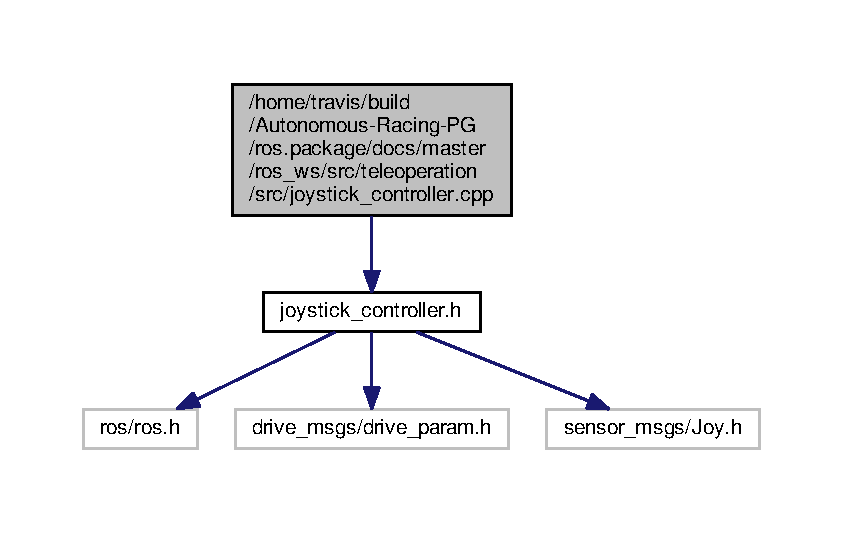
\includegraphics[width=350pt]{joystick__controller_8cpp__incl}
\end{center}
\end{figure}
\subsection*{Functions}
\begin{DoxyCompactItemize}
\item 
int \hyperlink{joystick__controller_8cpp_a3c04138a5bfe5d72780bb7e82a18e627}{main} (int argc, char $\ast$$\ast$argv)
\end{DoxyCompactItemize}


\subsection{Function Documentation}
\index{joystick\+\_\+controller.\+cpp@{joystick\+\_\+controller.\+cpp}!main@{main}}
\index{main@{main}!joystick\+\_\+controller.\+cpp@{joystick\+\_\+controller.\+cpp}}
\subsubsection[{\texorpdfstring{main(int argc, char $\ast$$\ast$argv)}{main(int argc, char **argv)}}]{\setlength{\rightskip}{0pt plus 5cm}int main (
\begin{DoxyParamCaption}
\item[{int}]{argc, }
\item[{char $\ast$$\ast$}]{argv}
\end{DoxyParamCaption}
)}\hypertarget{joystick__controller_8cpp_a3c04138a5bfe5d72780bb7e82a18e627}{}\label{joystick__controller_8cpp_a3c04138a5bfe5d72780bb7e82a18e627}


Definition at line 63 of file joystick\+\_\+controller.\+cpp.


\hypertarget{keyboard__controller_8cpp}{}\section{/home/travis/build/\+Autonomous-\/\+Racing-\/\+P\+G/ros.package/docs/master/ros\+\_\+ws/src/teleoperation/src/keyboard\+\_\+controller.cpp File Reference}
\label{keyboard__controller_8cpp}\index{/home/travis/build/\+Autonomous-\/\+Racing-\/\+P\+G/ros.\+package/docs/master/ros\+\_\+ws/src/teleoperation/src/keyboard\+\_\+controller.\+cpp@{/home/travis/build/\+Autonomous-\/\+Racing-\/\+P\+G/ros.\+package/docs/master/ros\+\_\+ws/src/teleoperation/src/keyboard\+\_\+controller.\+cpp}}
{\ttfamily \#include \char`\"{}keyboard\+\_\+controller.\+h\char`\"{}}\\*
Include dependency graph for keyboard\+\_\+controller.\+cpp\+:
\nopagebreak
\begin{figure}[H]
\begin{center}
\leavevmode
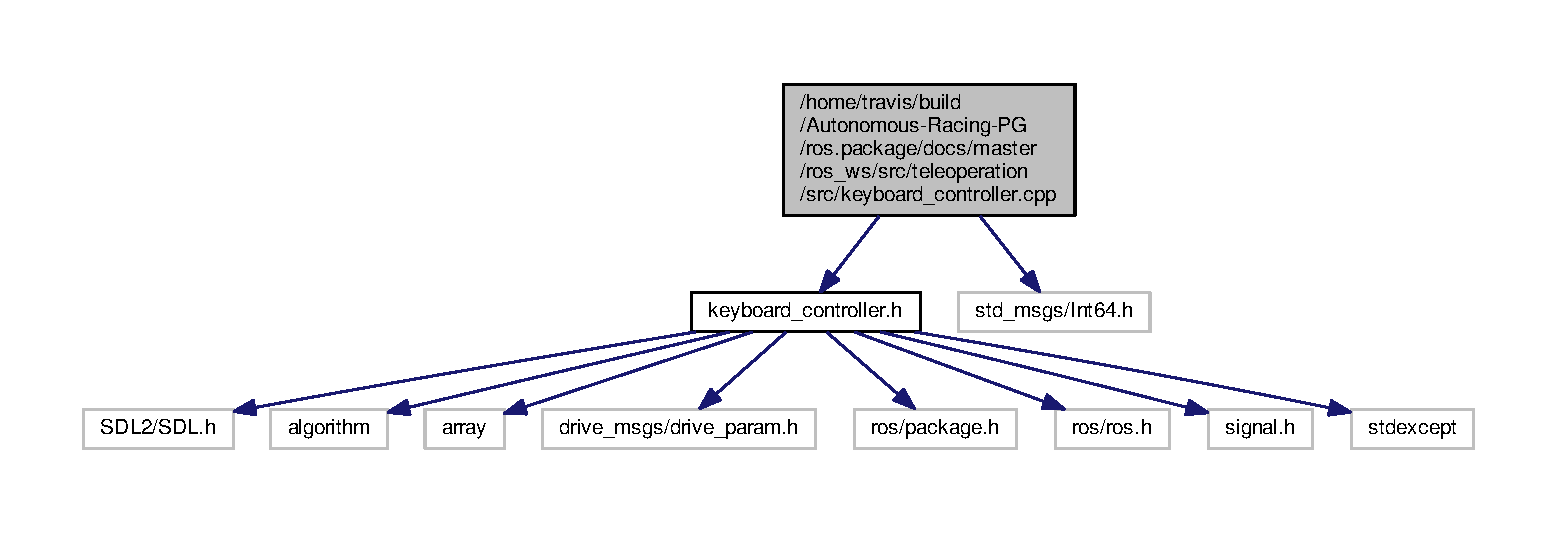
\includegraphics[width=350pt]{keyboard__controller_8cpp__incl}
\end{center}
\end{figure}
\subsection*{Functions}
\begin{DoxyCompactItemize}
\item 
double \hyperlink{keyboard__controller_8cpp_a215566526f35eabece78faa4ea465f24}{clamp} (double value, double lower, double upper)
\item 
double \hyperlink{keyboard__controller_8cpp_a9c2a2e4c6a836edf99a7e4107e3874ca}{map} (double value, double in\+\_\+lower, double in\+\_\+upper, double out\+\_\+lower, double out\+\_\+upper)
\item 
int \hyperlink{keyboard__controller_8cpp_a3c04138a5bfe5d72780bb7e82a18e627}{main} (int argc, char $\ast$$\ast$argv)
\end{DoxyCompactItemize}


\subsection{Function Documentation}
\index{keyboard\+\_\+controller.\+cpp@{keyboard\+\_\+controller.\+cpp}!clamp@{clamp}}
\index{clamp@{clamp}!keyboard\+\_\+controller.\+cpp@{keyboard\+\_\+controller.\+cpp}}
\subsubsection[{\texorpdfstring{clamp(double value, double lower, double upper)}{clamp(double value, double lower, double upper)}}]{\setlength{\rightskip}{0pt plus 5cm}double clamp (
\begin{DoxyParamCaption}
\item[{double}]{value, }
\item[{double}]{lower, }
\item[{double}]{upper}
\end{DoxyParamCaption}
)}\hypertarget{keyboard__controller_8cpp_a215566526f35eabece78faa4ea465f24}{}\label{keyboard__controller_8cpp_a215566526f35eabece78faa4ea465f24}


Definition at line 4 of file keyboard\+\_\+controller.\+cpp.



Here is the caller graph for this function\+:
\nopagebreak
\begin{figure}[H]
\begin{center}
\leavevmode
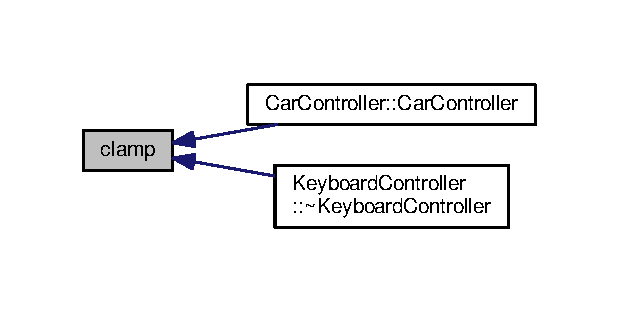
\includegraphics[width=271pt]{keyboard__controller_8cpp_a215566526f35eabece78faa4ea465f24_icgraph}
\end{center}
\end{figure}


\index{keyboard\+\_\+controller.\+cpp@{keyboard\+\_\+controller.\+cpp}!main@{main}}
\index{main@{main}!keyboard\+\_\+controller.\+cpp@{keyboard\+\_\+controller.\+cpp}}
\subsubsection[{\texorpdfstring{main(int argc, char $\ast$$\ast$argv)}{main(int argc, char **argv)}}]{\setlength{\rightskip}{0pt plus 5cm}int main (
\begin{DoxyParamCaption}
\item[{int}]{argc, }
\item[{char $\ast$$\ast$}]{argv}
\end{DoxyParamCaption}
)}\hypertarget{keyboard__controller_8cpp_a3c04138a5bfe5d72780bb7e82a18e627}{}\label{keyboard__controller_8cpp_a3c04138a5bfe5d72780bb7e82a18e627}


Definition at line 147 of file keyboard\+\_\+controller.\+cpp.

\index{keyboard\+\_\+controller.\+cpp@{keyboard\+\_\+controller.\+cpp}!map@{map}}
\index{map@{map}!keyboard\+\_\+controller.\+cpp@{keyboard\+\_\+controller.\+cpp}}
\subsubsection[{\texorpdfstring{map(double value, double in\+\_\+lower, double in\+\_\+upper, double out\+\_\+lower, double out\+\_\+upper)}{map(double value, double in_lower, double in_upper, double out_lower, double out_upper)}}]{\setlength{\rightskip}{0pt plus 5cm}double map (
\begin{DoxyParamCaption}
\item[{double}]{value, }
\item[{double}]{in\+\_\+lower, }
\item[{double}]{in\+\_\+upper, }
\item[{double}]{out\+\_\+lower, }
\item[{double}]{out\+\_\+upper}
\end{DoxyParamCaption}
)}\hypertarget{keyboard__controller_8cpp_a9c2a2e4c6a836edf99a7e4107e3874ca}{}\label{keyboard__controller_8cpp_a9c2a2e4c6a836edf99a7e4107e3874ca}


Definition at line 9 of file keyboard\+\_\+controller.\+cpp.



Here is the caller graph for this function\+:
\nopagebreak
\begin{figure}[H]
\begin{center}
\leavevmode
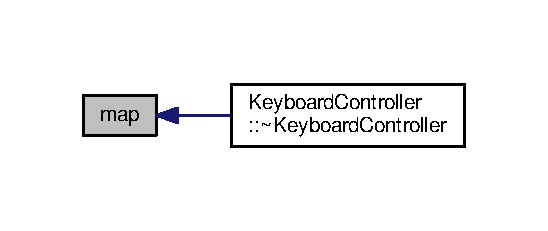
\includegraphics[width=263pt]{keyboard__controller_8cpp_a9c2a2e4c6a836edf99a7e4107e3874ca_icgraph}
\end{center}
\end{figure}



%--- End generated contents ---

% Index
\backmatter
\newpage
\phantomsection
\clearemptydoublepage
\addcontentsline{toc}{chapter}{Index}
\printindex

\end{document}
